\chapter{Background}
\label{chpt:2}
\paragraph{}
This chapter provides an overview of the different task and concepts needed to perform relation extraction in a multilingual setup. Some concepts, like word representation~(Section \ref{sec:word_embedding}) are at the core of NLP, while others are more general machine learning techniques (Section~\ref{sec:nn},~\ref{sec:transfer_learning} and \ref{sec:zero_learning}), others instead are both general and have a very high usage in NLP due to their nature (Section \ref{sec:sequence_modeling}). 


% In the next Chapter we will describe more the task of relation extraction, and present how Natural Language Understanding, a sub-field of NLP that deals with machine reading comprehension, which can be used for relation extraction.

% \section{Introduction}
% Natural Language Processing solutions span form rule based systems~\citep{brill-1992-simple, nebhi2013rulere}, to statistical approaches~\citep{skounakis2003hierarchical}, and also to neural networks~\citep{pawar-etal-2017-end}.

\section{Neural Networks}
\label{sec:nn}

\paragraph{}
A Neural Network (NN) is a computational model inspired by networks of biological neurons, wherein the neurons compute output values from inputs. The simplest form of neural network is the feed forward neural network, in which the information flows only in one direction, and there is no recurrent connection between the nodes. Neural networks try to approximate some function $f^{*}$ by defining a mapping $y = f(x; W)$ for an input $x$ by  learning the value of the parameters $W$ that yield the best function approximation. A neural network is called network because it contains multiple layers of artificial neurons. The artificial neuron is the building block of neural networks.

A neuron is defined by an input $x$, a set of weights $W$, a bias $b$, and an activation function $g$. The activation function should be differentiable, since to actually learn, we need to compute derivatives. With $x, W \in \mathbb{R}^{n\times1}$, $b \in \mathbb{R}$. The output $y$ is defined as: 

\begin{equation}
    y = g(W^{\intercal} x + b)
\end{equation}


Feed forward neural networks are composed by various layers, each layer contains some neurons. The formal definition is very similar to the one of the neuron. To simplify the notation, we will include the bias term in the weights matrix, and have an extra element $x_0 = 1$ in the input $x$. Given a feed forward neural network with $L$ layers, the forward propagation is: 

\begin{equation}
\begin{split}
    %y = f^{k}(W_{k}^{\intercal} * \dots f^{2}(W_{2}^{\intercal} * f^{1}(W_{1}^{\intercal} * x)) \dots)
    z^i & = W^{i-1}a^{i-1} \\
    a^{i} & = g(z^i) \\
    y & = a^L g(z^L) \\
\end{split}
\end{equation}

Where $g$ is an activation function, $a^i$ is the activation of layer $i$, and $a^0 = x$. The weight matrix $W_i$ controls the projection from layer $i$ to layer $i+1$. Given a network with $s_i$ units in layer $i$, and $s_{i+1}$ in layer $i+1$ the weight matrix $W_i \in\mathbb{R}^{(s_{i+1})\times (s_i + 1)} $. 

As in other machine learning algorithms, we have to learn the parameters of our neural network. We have a cost function, or objective function, $J(\theta)$ that we try to minimize. Given a neural network $h_\theta$, we compute our cost function as a sum of the error function  $\mathcal{L}$ for all the examples. The error function computes the difference between the predicted value $\hat{y} = h_{\theta}(x)$ and the actual value $y$. We also have a regularizer term $\Omega$ that is weighted by the hyperparameter $\lambda$:

\begin{equation}
    \min_{\theta} J(\theta) = - \frac{1}{N} \sum_{1}^{N} \mathcal{L}(y_i, \hat{y_i}) + \lambda \Omega_\theta
\end{equation}

Now that we have defined what is the goal of our neural network, we can start performing the training. %The learning algorithm for neural network is called backpropagation, from backward propagation of errors. 
The weights $\theta$ in the network are the only parameters that can be modified to make the cost function $J$ as low as possible; thus we can minimize $J$ by using an iterative process of gradient descent, for which we need to calculate the gradient for the cost function with respect to the network parameters.  As each network consists of various layers, computing the gradient of the loss function w.r.t the parameters $\frac{\partial J}{\partial \theta}$ is non-trivial. To estimate the gradient, we use a an algorithm called backpropagation~\citep{rumelhart1988learning}, from backward propagation of errors. As the name implies, backpropagation starts computing the gradients from the output of the networks and moves backward to the input through all layers. First, we need to compute the derivative of $J(\theta)$ w.r.t the output, this will be our $\partial^{L}$, then go backward:



%Equation~\ref{eq:backpropagation}. 

\begin{equation}
\begin{split}
    \partial^{L} & = \frac{\partial}{\partial y} \mathcal{L}(y, \hat{y}) \\
    \partial^i &= {\theta^{i}}^\intercal \partial^{i+1} \odot \left(\frac{\partial}{\partial z^{i}} g(z^i)\right)
\end{split}
\label{eq:backpropagation}    
\end{equation}

For each layer, the computed gradients are then used to update the corresponding parameters using gradient descent.

\section{Sequence Modeling}
\label{sec:sequence_modeling}


\paragraph{}
Due to the inherent nature of natural language almost all NLP tasks deal with sequences. For example, in speech recognition, we have the input audio which is a sequence of phonemes that will be recognised and used to produce a transcript. Likewise, in machine translation we have as input a sequence of words in a source language and the machine has to generate a new sequence of words with the same meaning of the input sequence but in a target language.


Traditional neural networks are not designed to deal with the temporal information of sequences in an efficient way. A way to handle this problem is to introduce the notion of a dynamical system. In the dynamical system, there is a state which carries information about past inputs. Typically, we make what is called a Markov assumption; that means that all the information regarding the past and current inputs required to estimate a future state is succinctly contained in the current state. A Recurrent Neural Network (RNN) is a particular type of dynamical system.

\subsection{Recurrent Neural Network}
\paragraph{}
The most elementary neural network for sequential input is the recurrent neural network~\citep{elman1990finding}. Elman proposes a recurrent network based on the idea introduced by~\citet{jordan1986} which proposes a network with recurrent connections from the output to the input; these are one-to-one connections that are used to associate a static pattern with a serially ordered output pattern. Elman modifies the network by moving the recurrent connection. Instead of having the output connected with the input, Elman adds additional units at the input level, these units are called ``\textit{context units}" and are connected to the hidden layer. Context units are also “hidden” in the sense that they interact exclusively with other nodes internal to the network, and not the outside world. 

In Figure~\ref{fig:rnn} we can have a look at how a RNN works. The network $A$ takes in input $x_t$ and produces an output $h_t$, a loop enables the information to flow from the previous step to the current, allowing the prediction to be affected by the last state of the network. A more effective way to think about RNNs is by unrolling them (right side of Figure~\ref{fig:rnn}). We can formally define $A$ as:

\begin{figure}[t]
        \centering
        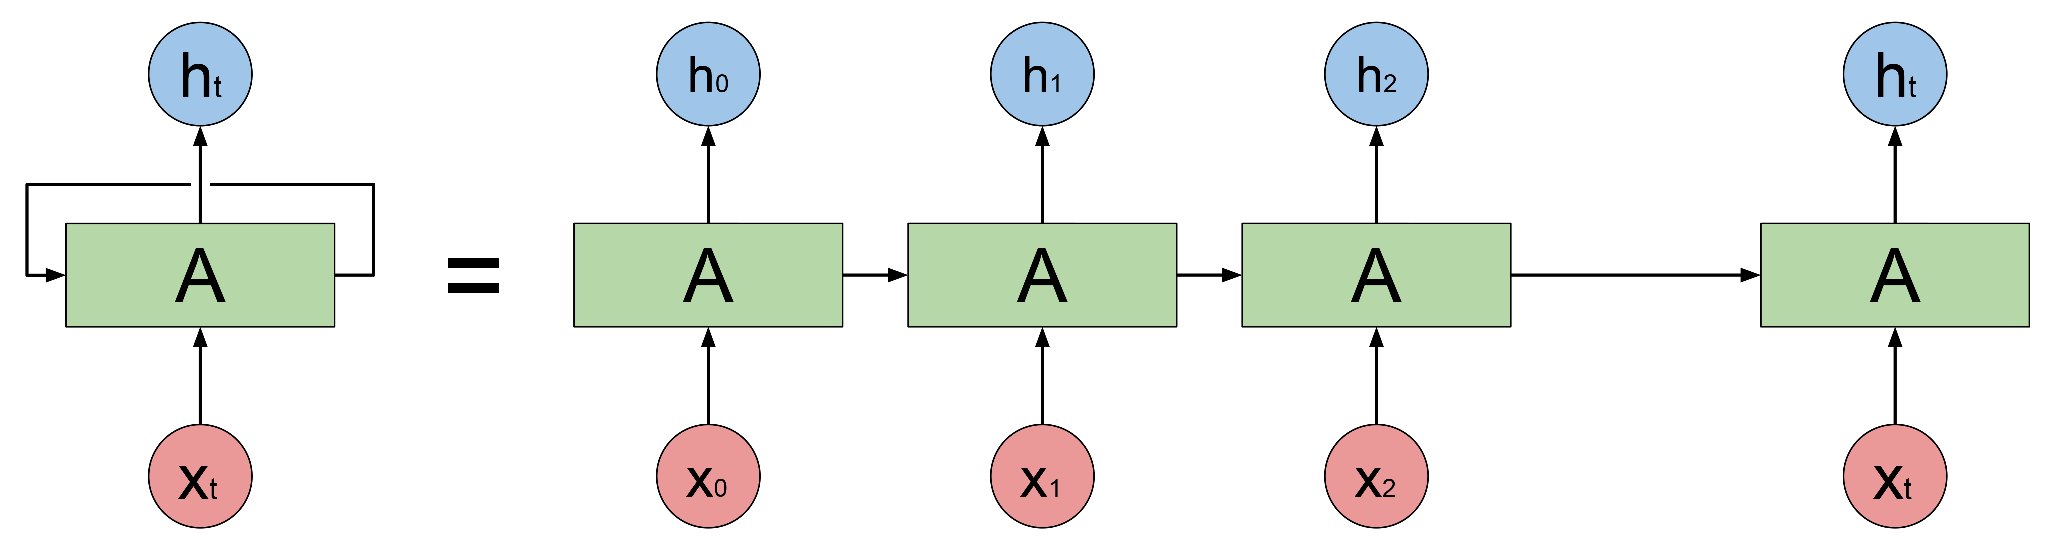
\includegraphics[width=0.9\textwidth]{images/RNN.pdf}
        \caption{RNN unrolling. On the left a compact representation of RNNs, on the right the same RNN can be unrolled}
        \label{fig:rnn}
\end{figure}%

\begin{equation}
\begin{split}
    h_t & = f_W(h_{t-1}, x_t) \\
    y_t & = g_{\theta}(h_t)
\end{split}
\label{eq:generic_rnn}
\end{equation}

Where, $h_t$ is the new state, $f_W$ and $g_\theta$ are functions with parameters $W$ and $\theta$ respectively, $h_{t-1}$ is the previous state, $x_t$ is the current input, and $y_t$ is the output at the \textit{t-th} step.
The vanilla RNN is defined using a neural network with $\tanh$ as activation function, so we will have:

\begin{equation}
\begin{split}
    h_t & = \tanh\left(W_h \cdot h_{t-1} + W_x \cdot x_t\right)\\
        & = \tanh\left([W_h, W_x] \cdot \begin{bmatrix}
           h_{t-1} \\
           x_t
         \end{bmatrix}\right)\\
         & = \tanh\left(W \cdot \begin{bmatrix}
           h_{t-1} \\
           x_t
         \end{bmatrix}\right)
\end{split}
\end{equation}

Where $W_h$, $W_x$ are weights for the hidden and input respectively. 

\paragraph{}
RNN are able to manage variable length of input and output sequences, we can have different types of RNN according to these sizes. Given a sequence $x$ of length $l_x$, and a desired output sequence $y$ with length $l_y$, we can define the following types (visually represented in Figure~\ref{fig:rnn_types}):

\begin{enumerate}[a), noitemsep]
    \item One-to-One: $l_x = l_y = 1$, this is a traditional neural network;
    \item One-to-Many: $l_x = 1, l_y > 1$, this is the case for sequence generation;
    \item Many-to-One: $l_x > 1, l_y = 1$, for sequence classification;
    \item Many-to-Many: $l_x = l_y > 1$, for sequence labeling;
    \item Many-to-Many: $l_x \neq l_y, l_x > 1, l_y > 1$, also referred to as sequence-to-sequence~\citep{sutskever2014sequence}, or encoder-decoder~\citep{cho-etal-2014-learning}. Given an input sequence, the encoder process it and generates a dense representation which is used to initialize the decoder that will produce the output sequence. This is elaborated in Section~\ref{sec:encoder_decoder}
\end{enumerate}

\begin{figure}
\begin{tcbitemize}[
    raster columns=3,
    raster halign=center,
    raster every box/.style={blankest}
    ]
\mysubfig{One-to-One}{images/one_to_one.pdf}
\mysubfig{One-to-Many}{images/one_to_many.pdf}
\mysubfig{Many-to-One}{images/many_to_one.pdf}
\mysubfig{Many-to-Many}{images/many_to_many.pdf}
\mysubfig{Many-to-Many}{images/many_to_many_s2s.pdf}
\end{tcbitemize}

\caption{Different types of RNN}
\label{fig:rnn_types}
\end{figure}

% \begin{figure} [H]
% \centering
% \begin{tabular}{cccc}
% 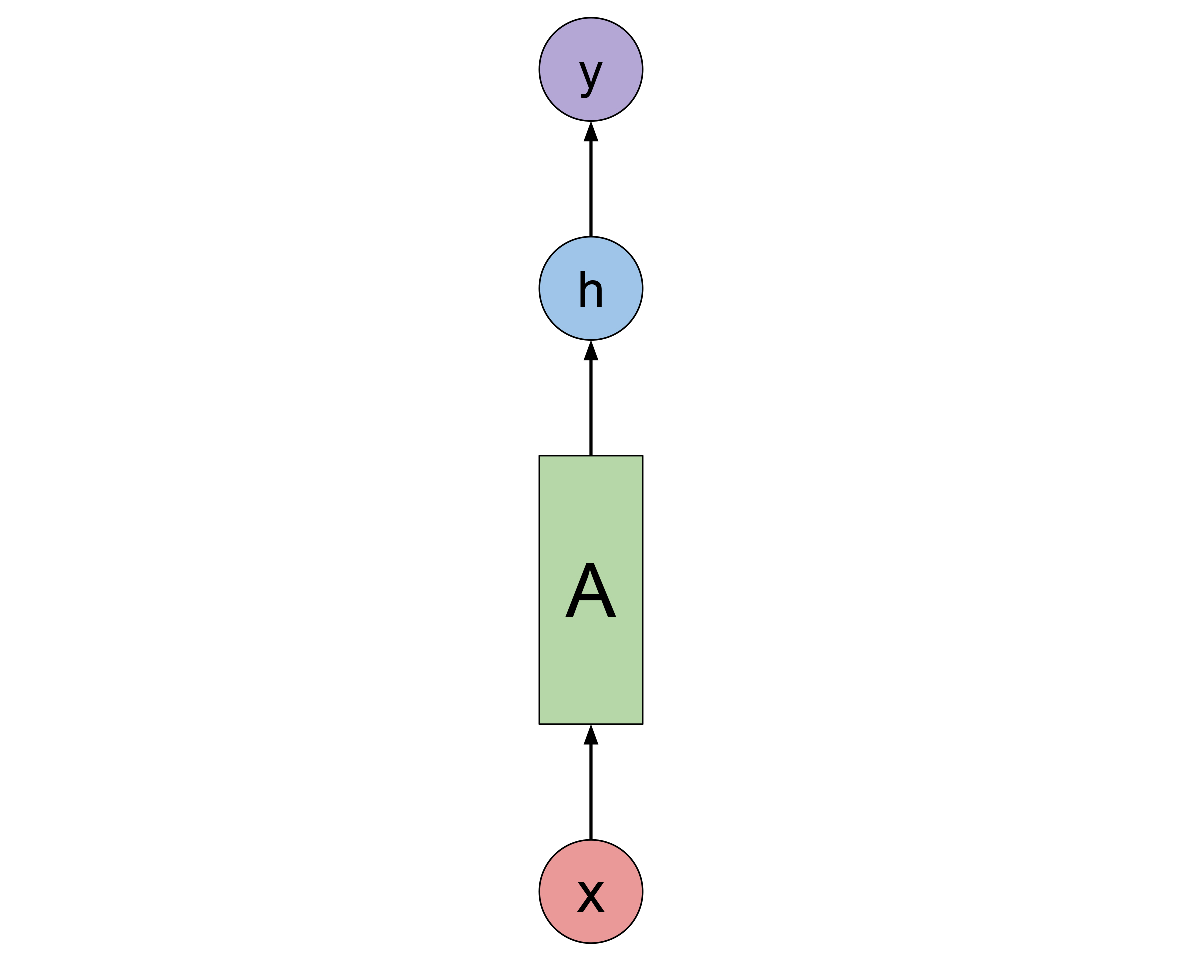
\includegraphics[width=0.3\textwidth]{images/one_to_one.pdf} &
% 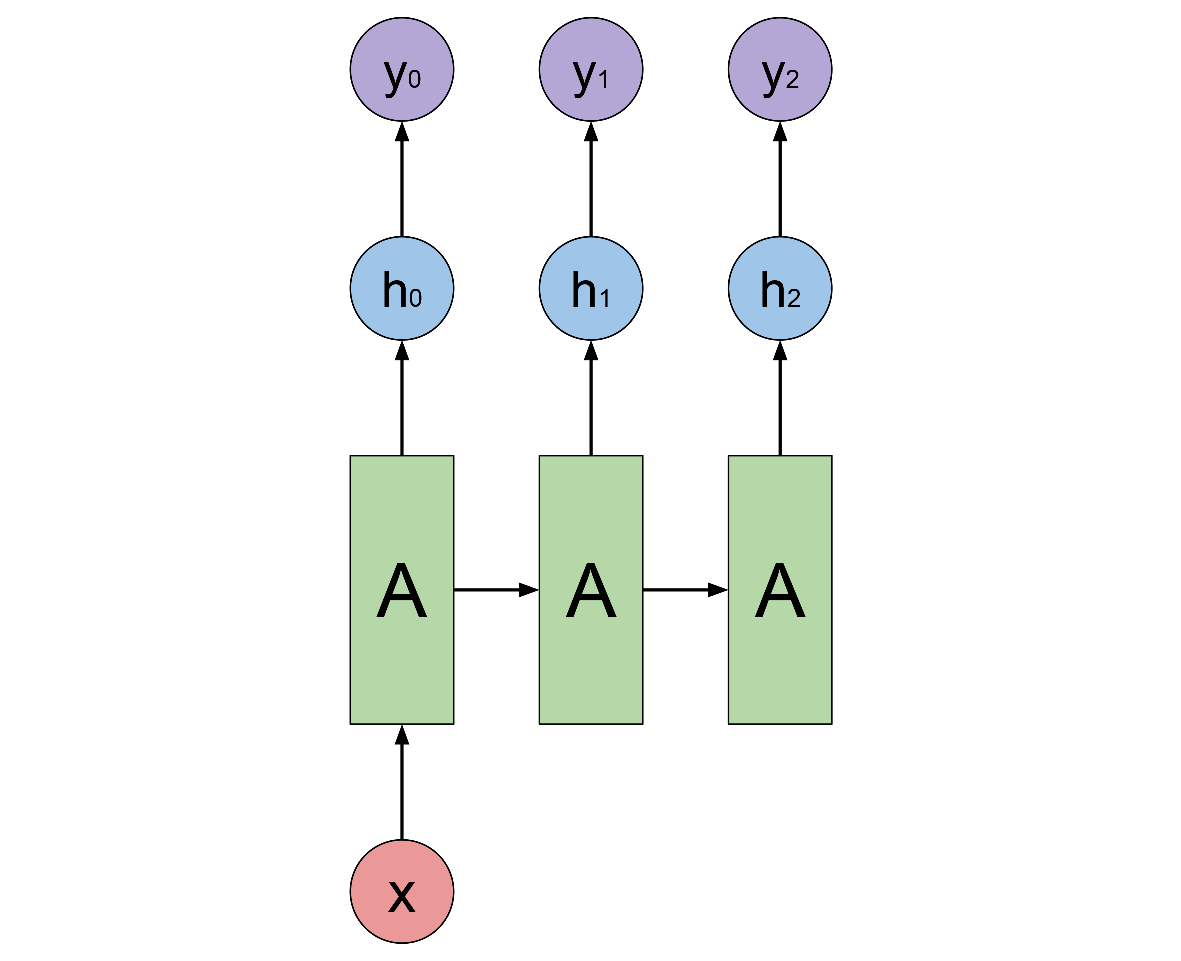
\includegraphics[width=0.3\textwidth]{images/one_to_many.pdf} &
% 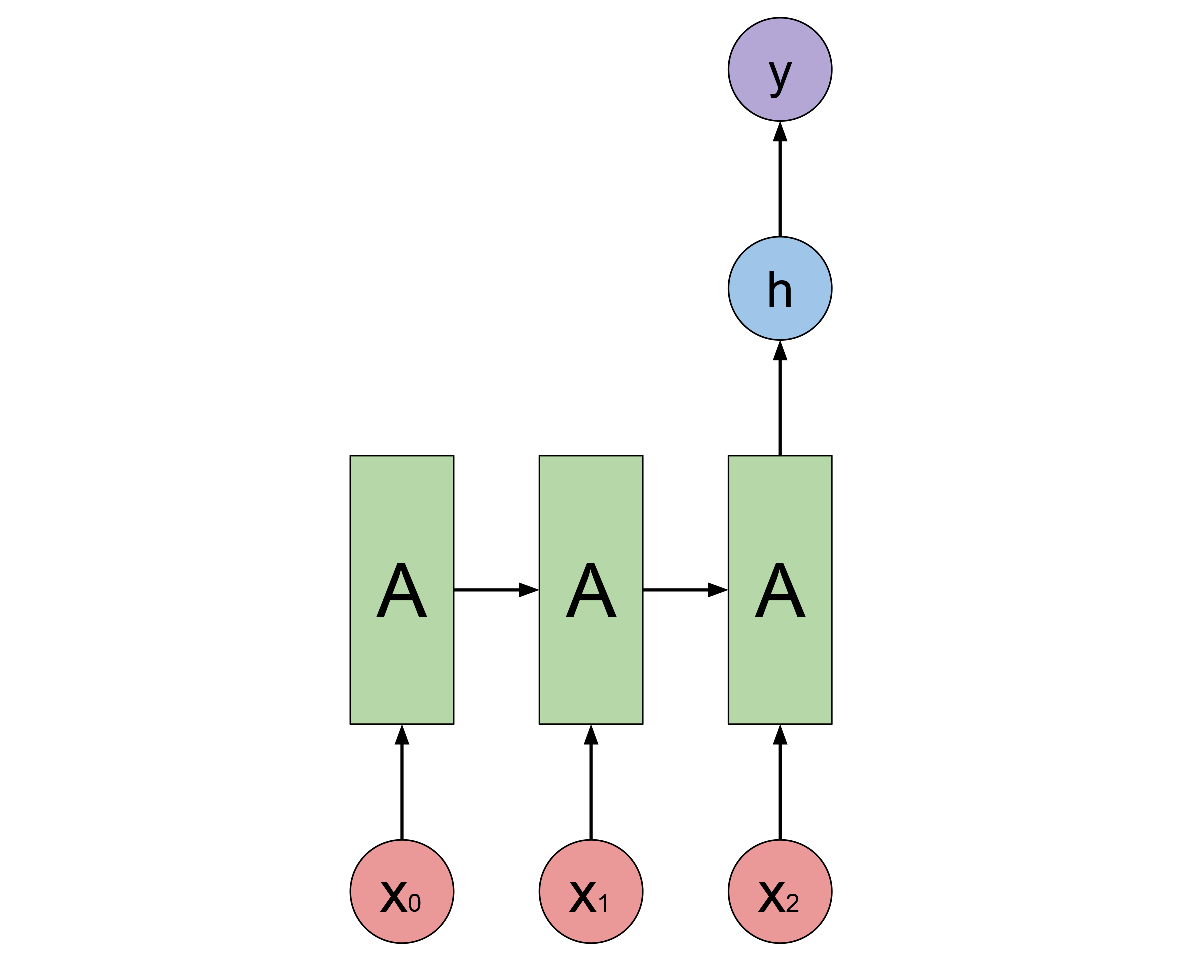
\includegraphics[width=0.3\textwidth]{images/many_to_one.pdf} \\
% \textbf{(a)}  & \textbf{(b)} & \textbf{(c)}  \\[6pt]
% \end{tabular}
% \begin{tabular}{cccc}
% \includegraphics[width=0.3\textwidth]{example-image-a} &
% \includegraphics[width=0.3\textwidth]{example-image-b} \\
% \textbf{(d)}  & \textbf{(e)}  \\[6pt]
% \end{tabular}
% \caption{ \textbf{(a)} Some text
% \textbf{(b)} Some text
% \textbf{(c)} Some text
% \textbf{(a)} Some text
% \textbf{(b)} Some text}
% \label{fig:peroxide}
% \end{figure}

% \begin{table}[ht]
% \caption{A table arranging  images}
% \centering
% \begin{tabular}{*{4}{|m{0.24\textwidth}}|}
% \hline
% 1 & 2 & 3 & 4  \\
% \hline
%  \begin{center}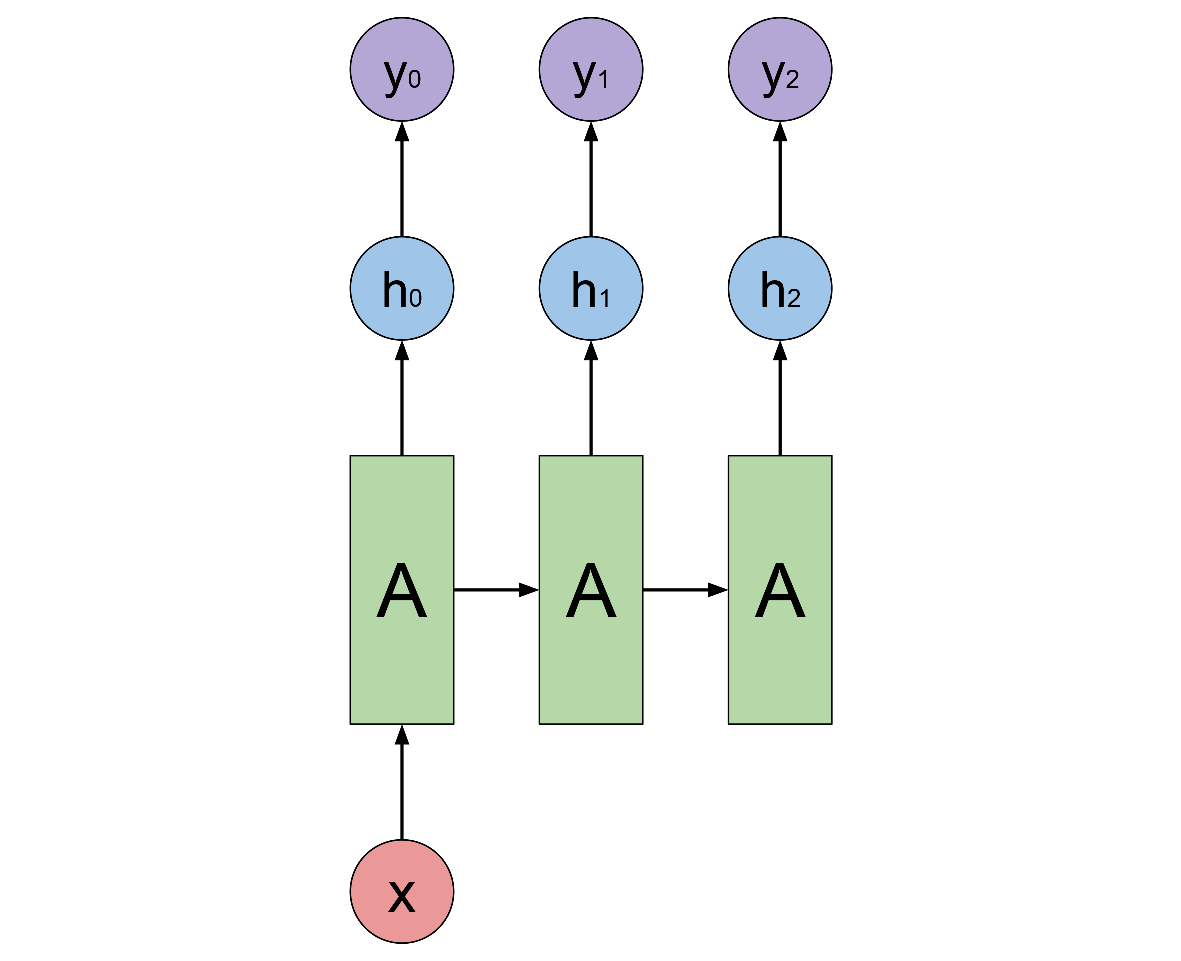
\includegraphics[height=0.1\textwidth]{images/one_to_many.pdf} \end{center} &
% \begin{center}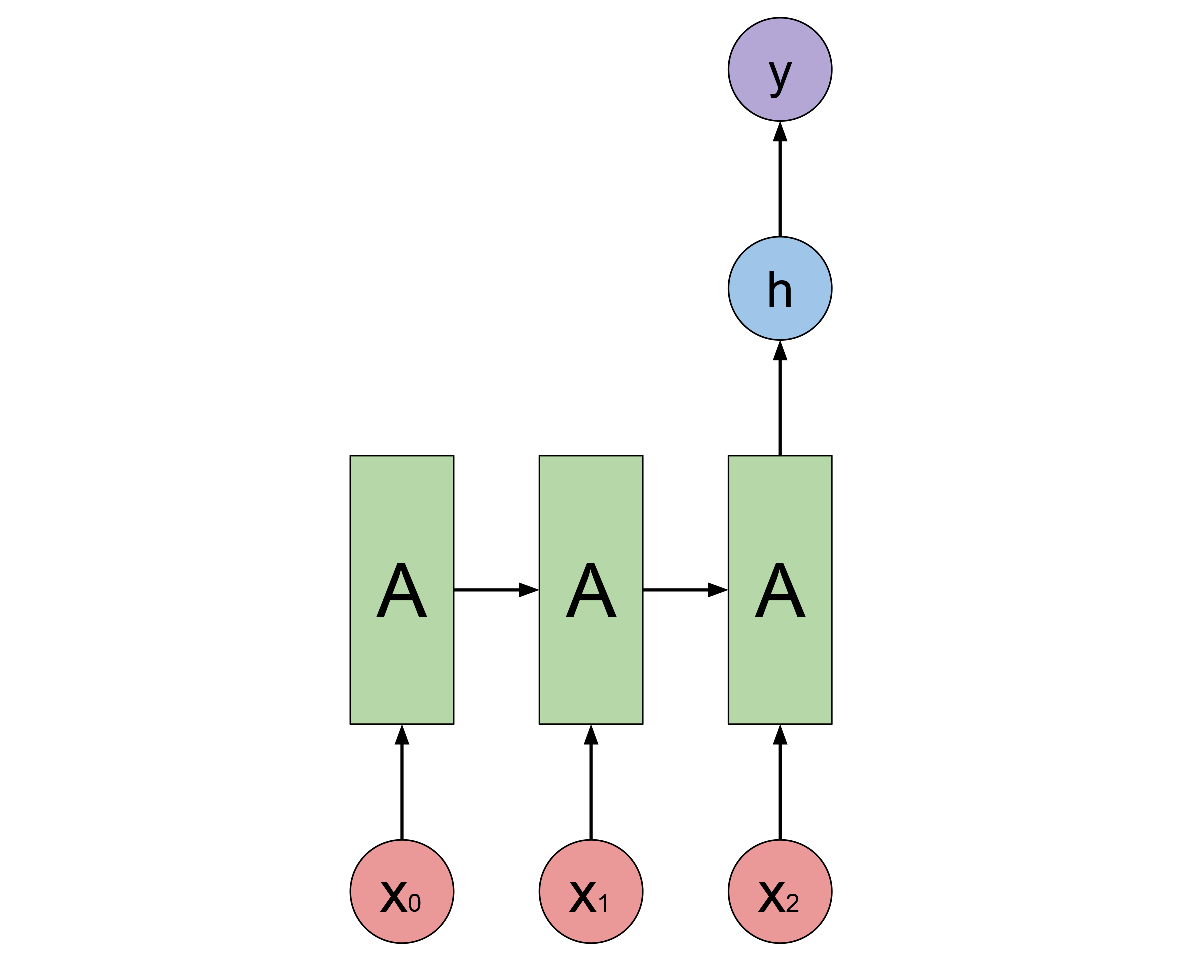
\includegraphics[height=0.1\textwidth]{images/many_to_one.pdf} \end{center} &
% \begin{center}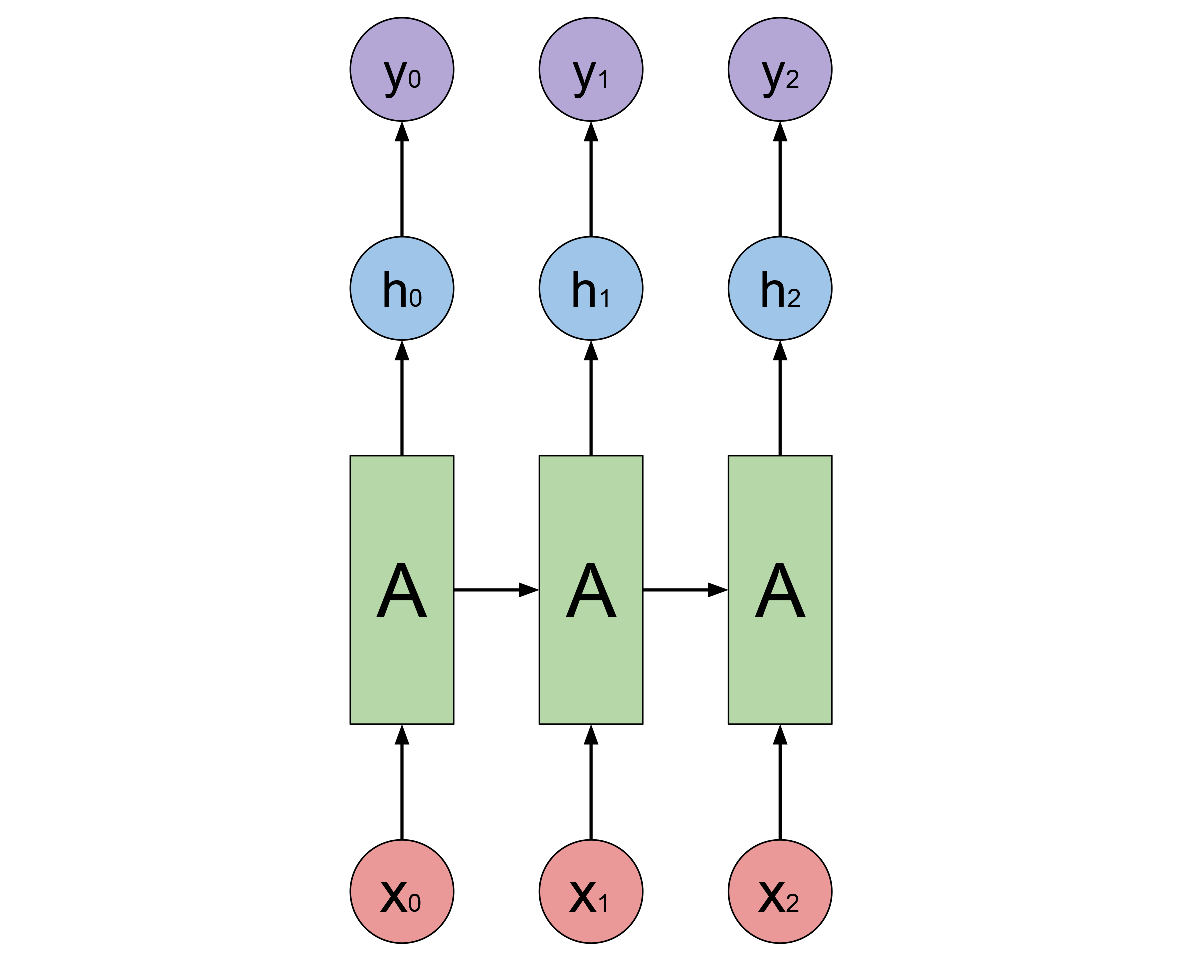
\includegraphics[height=0.1\textwidth]{images/many_to_many.pdf} \end{center} & \begin{center}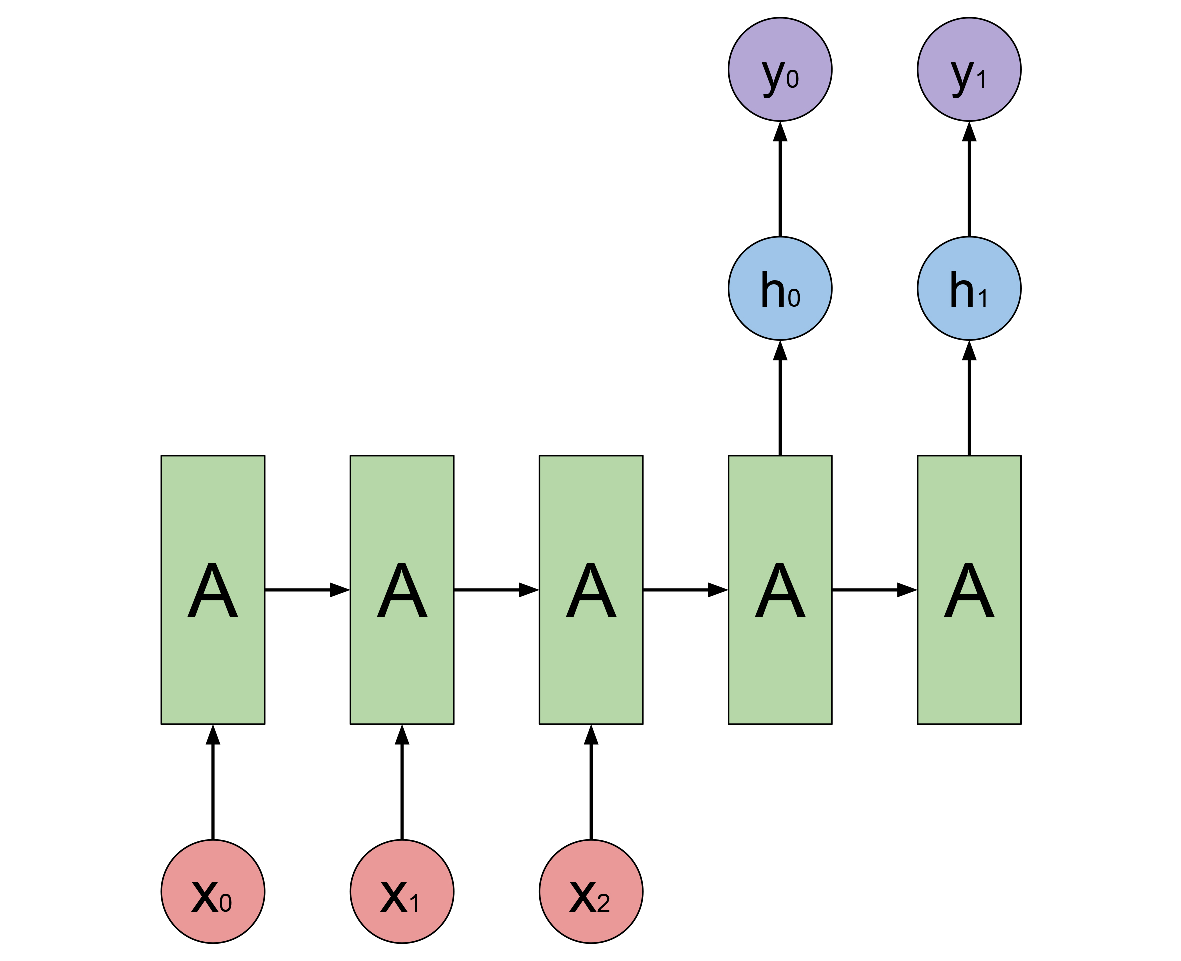
\includegraphics[height=0.1\textwidth]{images/many_to_many_s2s.pdf} \end{center} \\
% \hline
% \end{tabular}
% \label{tab:gt}
% \end{table}

% \begin{table}[ht]
% \caption{A table arranging  images}
% \centering
% \begin{tabular}{*{4}{|m{0.24\textwidth}}|}
% \hline
% This is some text & \begin{center}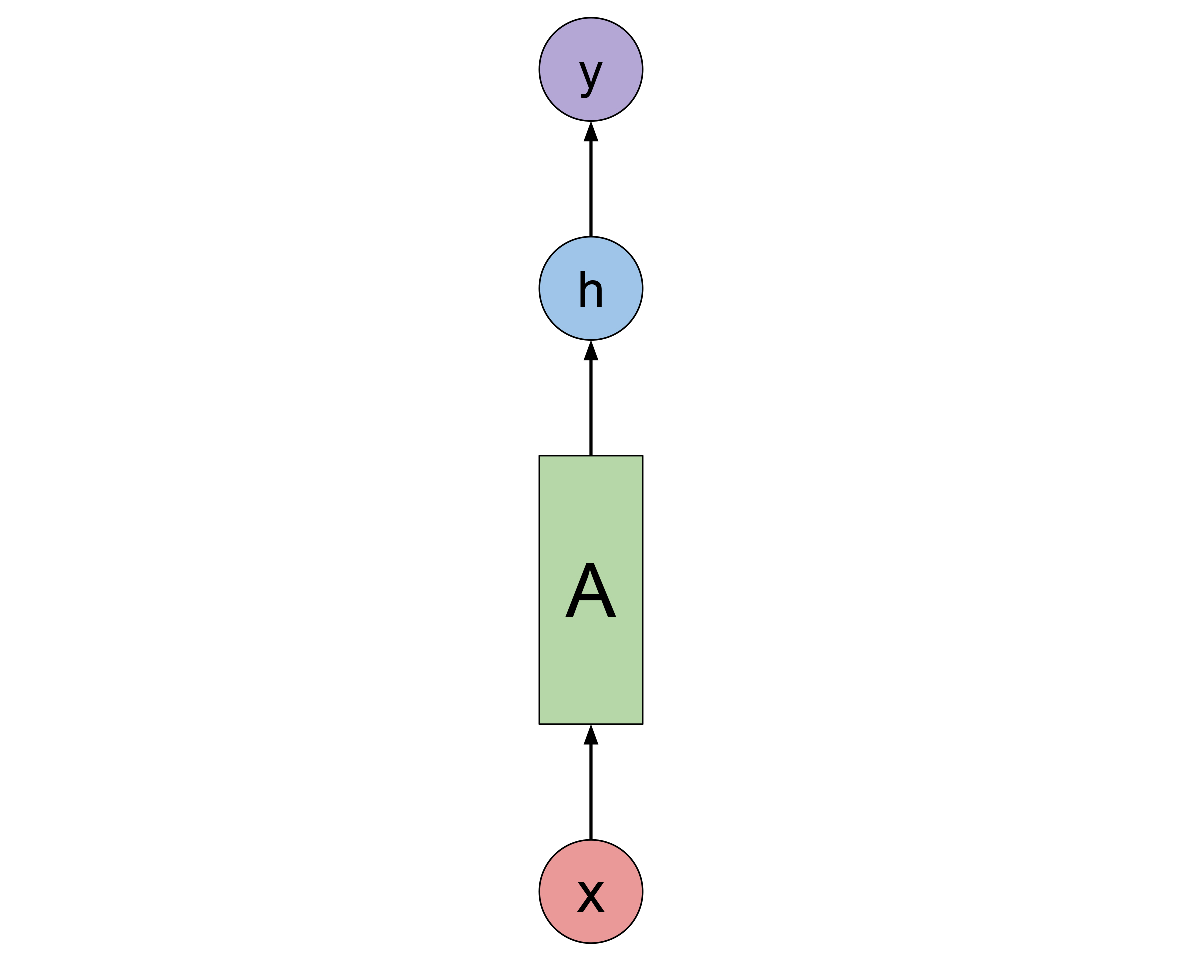
\includegraphics[height=0.2\textwidth]{images/one_to_one.pdf}\end{center} & This is some text & \begin{center}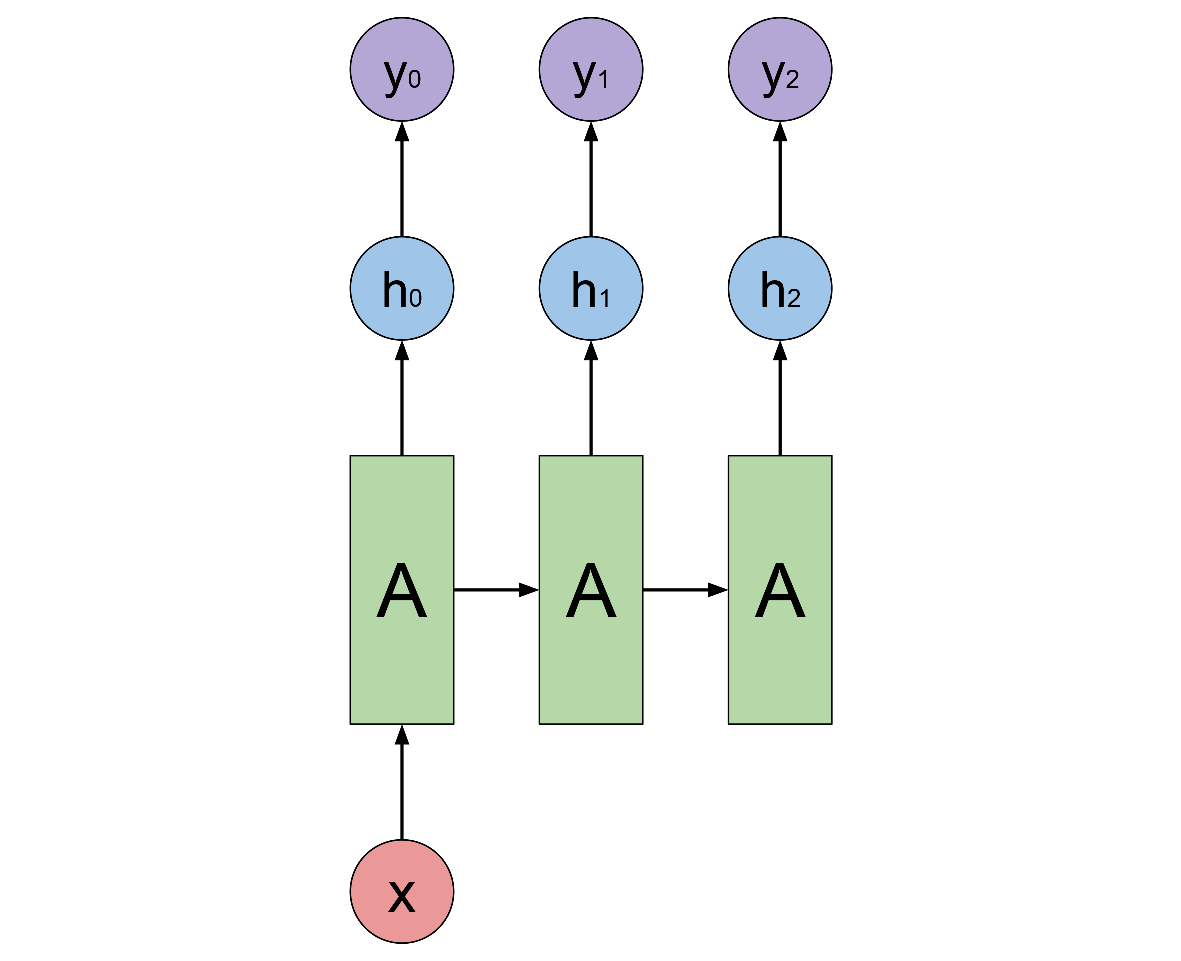
\includegraphics[height=0.2\textwidth]{images/one_to_many.pdf}\end{center} \\
% \hline
% This is some text & \begin{center}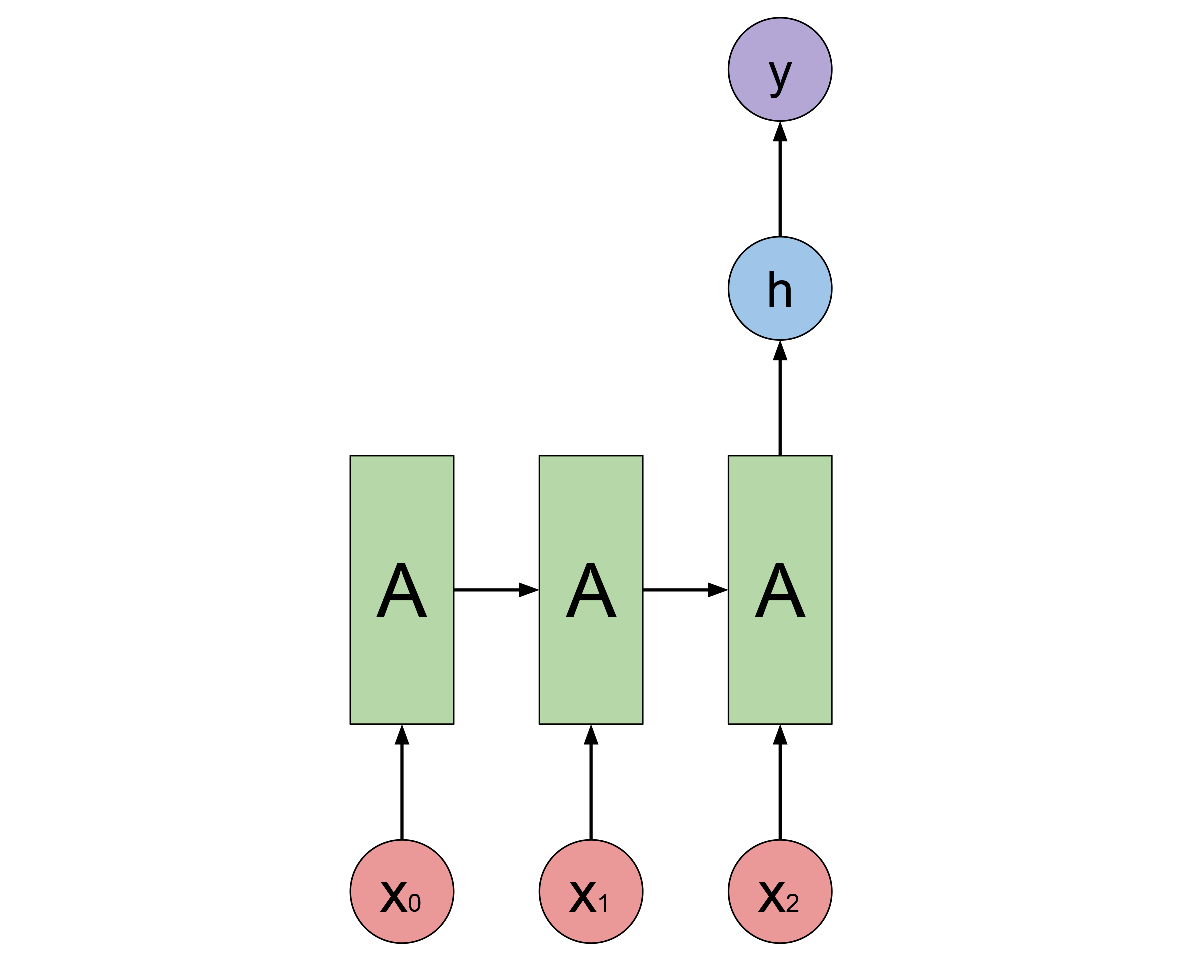
\includegraphics[height=0.2\textwidth]{images/many_to_one.pdf}\end{center} & This is some text & \begin{center}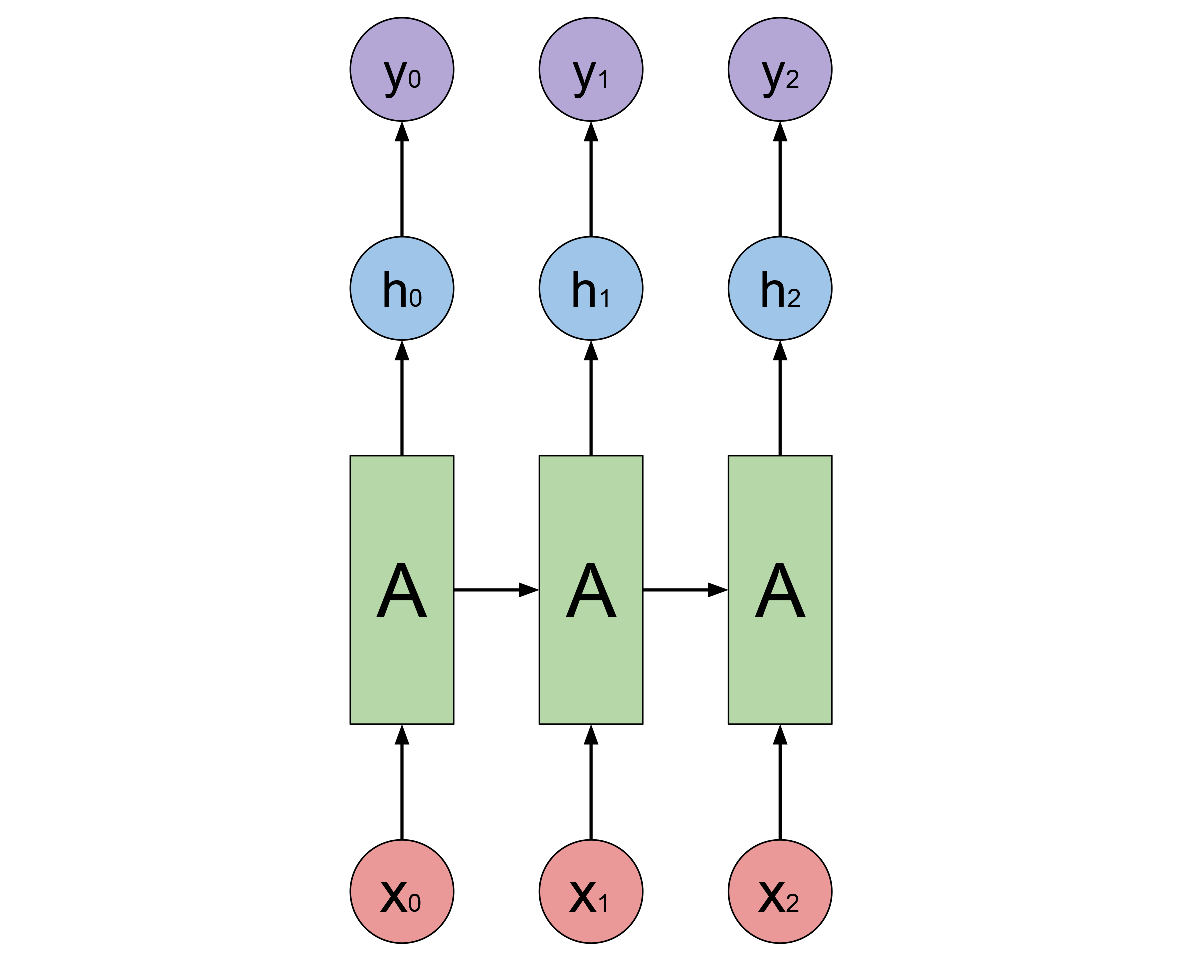
\includegraphics[height=0.2\textwidth]{images/many_to_many.pdf}\end{center} \\
% \hline
% This is some text & \begin{center}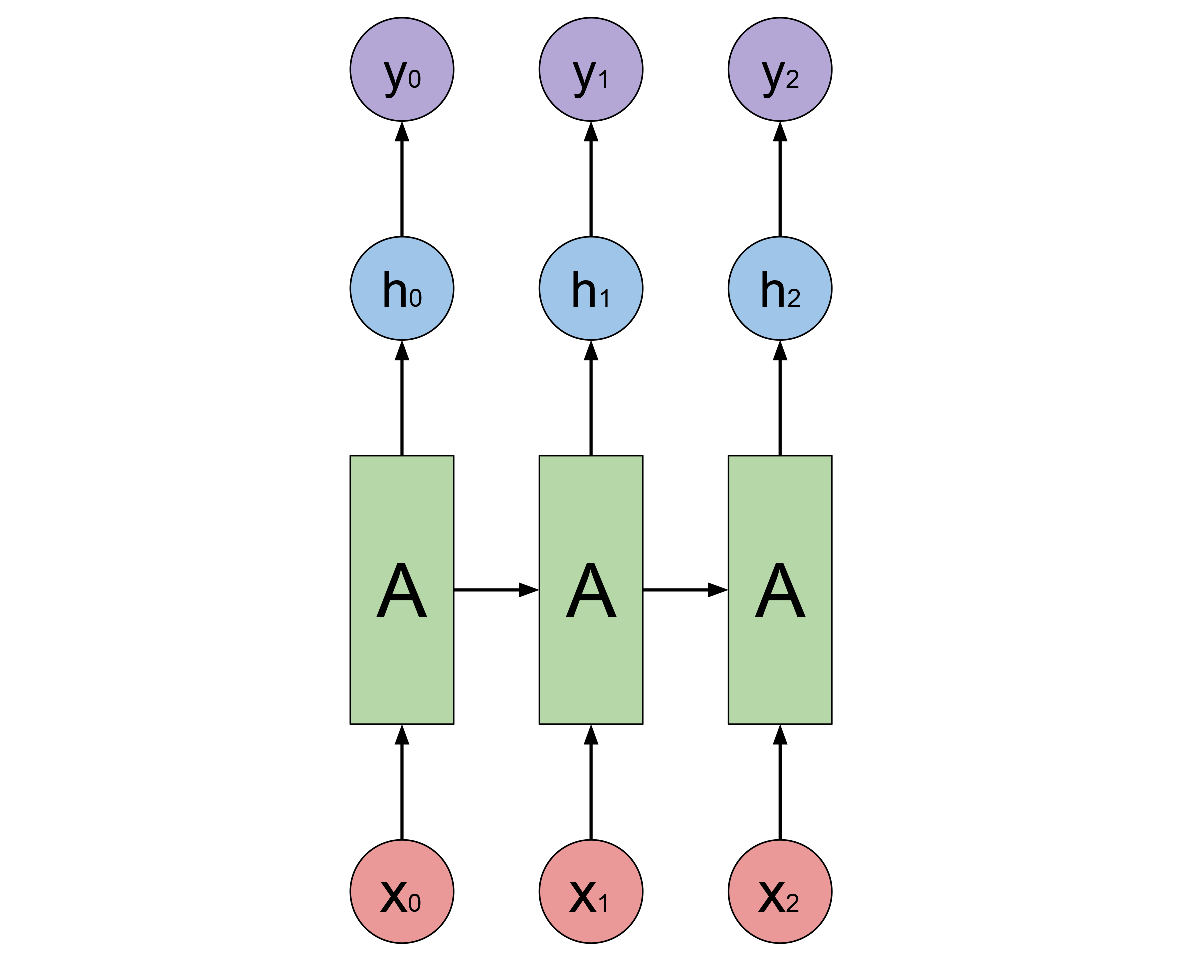
\includegraphics[height=0.2\textwidth]{images/many_to_many.pdf}\end{center} & & \\
% \hline
% \end{tabular}
% \label{tab:gt}
% \end{table}

% \begin{itemize}
%     \item One-to-One if $l_x = l_y = 1$, this is a traditional neural network;
%     \item One-to-Many if $l_x = 1, l_y > 1$, this is the case for sequence generation;
%     \item Many-to-One if $l_x > 1, l_y = 1$, for sequence classification;
%     \item Many-to-Many if $l_x = l_y > 1$, for sequence labeling;
%     \item Many-to-Many if $l_x \neq l_y, l_x > 1, l_y > 1$, for sequence-to-sequence tasks.
% \end{itemize}

We can also have bidirectional RNNs~\citep{Schuster1997BiRNN} (BiRNN). A BiRNN is composed of two RNNs, one looks at the sequence starting from the end while the other from the beginning as usual. The output at each step of a bidirectional RNN is the concatenation of the hidden states for that time step. In a BiRNN we have a left-to-right hidden state (or forward state) $\overrightarrow{h_t} = RNN(x_t, \overrightarrow{h}_{t-1})$, a right-to-left one (or backward state) $\overleftarrow{h_t} = RNN(x_t, \overleftarrow{h}_{t-1})$, and the output hidden state $h_t$ is defined as the concatenation of the directional hidden layers: $h_t = [\overrightarrow{h_t}, \overleftarrow{h_t}]$. The advantage of having bidirectional information is quite clear, the model is able to represent also future information, so the current decision is affected by both past and future.

Recurrent networks have various advantages over traditional networks. These include the ability to process sequences of any length, the size of the model does not increase with the size of the input, and most important, the computation takes into consideration historical information that should allow RNNs to learn long-term dependencies. Unfortunately, they also have some drawbacks. They are computationally more intensive, and even if they can work with sequences of any length and pass information through time, this information transfer starts to become less effective for longer sequences, which means they struggle to model longer-term dependencies. That is caused by the vanishing/explosion of the gradient, a significant issue in vanilla RNN. 

The vanishing gradient problem was first studied by~\cite{Hochreiter:91, bengio1994vanishing}. The problem occurs when we try to train a neural network model using gradient-based optimisation techniques, the backpropagation of the loss function with respect to the weights tends to vanish. This is a consequence of what happens during forward propagation; the hidden state is multiplied several times with the weight matrix, once per time step. So, during backpropagation, this leads to the gradients being multiplied by the same values many times, causing the gradient values to either explode, i.e. grow extremely large or vanish, i.e. become very small, making the model unable to learn. In RNNs this translates to that is very tough to allow the error to flow from the further in time inputs to the ones at the beginning, thus creating difficulties to train the early stages of the RNN and reducing the ability to learn long-term dependencies due to insufficient weight changes. A solution to this problem are the LSTMs.

% \begin{equation}
% \begin{split}
%     h_t & = tanh(W_{h} * h_{t-1} + W_x * x_t) \\
%     y_t & = W_y * h_t
% \end{split}
% \end{equation}

% \begin{figure*}[ht!]
%     \centering
%     \begin{subfigure}[t]{0.3\textwidth}
%         \centering
%         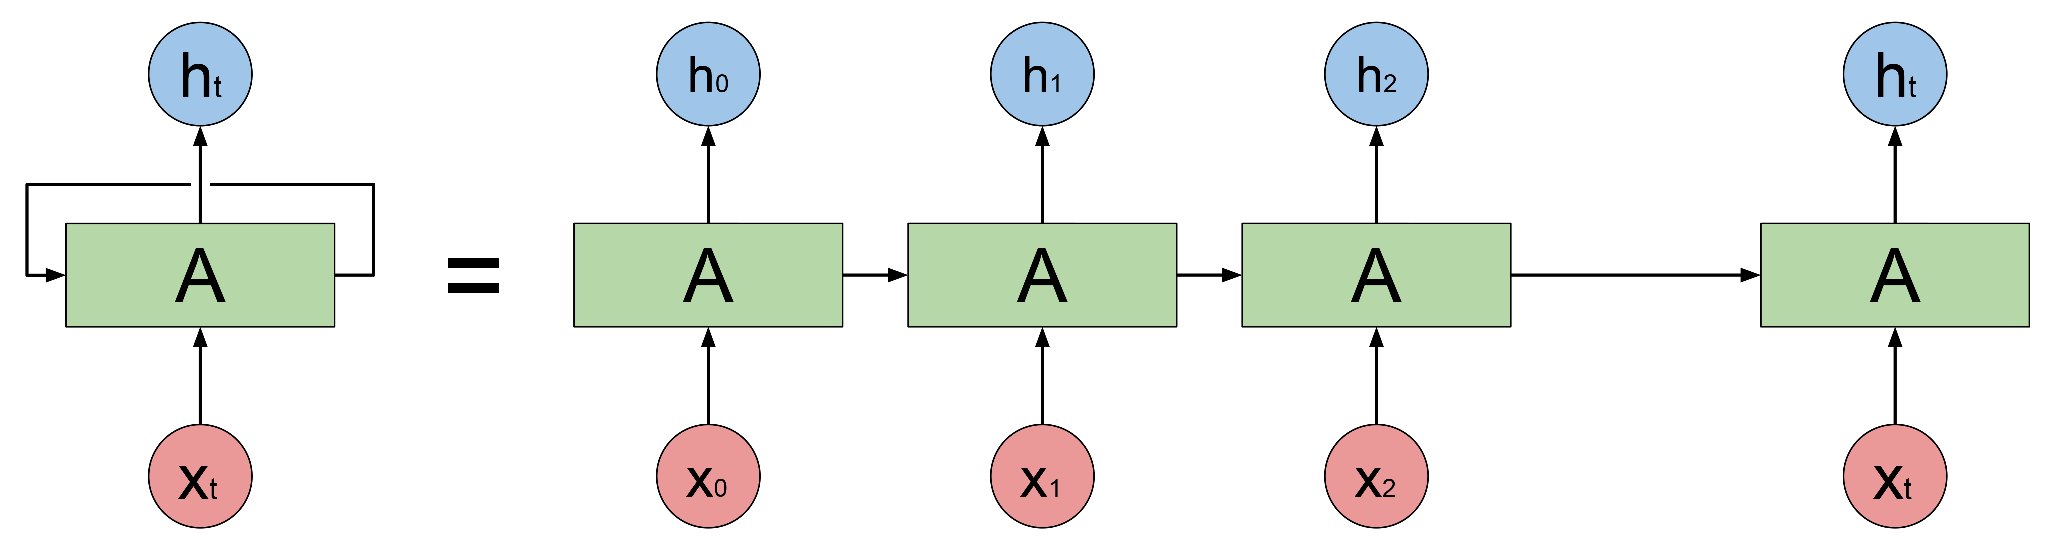
\includegraphics[width=0.7\textwidth]{images/RNN.png}
%         \caption{}
%         \label{subfig:rnn}
%     \end{subfigure}%
%     ~ 
%     \begin{subfigure}[t]{0.7\textwidth}
%         \centering
%         \includegraphics[width=\textwidth]{images/RNN-unrolled_only.png}
%         \caption{}
%         \label{subfig:rnn_unrolled}

%     \end{subfigure}
%     \caption{Different views of a recurrent neural network. In Figure~\ref{subfig:rnn} we have the compact view. Figure~\ref{subfig:rnn_unrolled} shows the same architecture but unrolled. Image credit: Christopher Olah}
%     \label{fig:rnn}
% \end{figure*} 


\subsection{Long Short Term Memory}
\label{sec:lstm}

\begin{figure}[]
    \centering
    \begin{subfigure}[t]{0.5\textwidth}
        \centering
        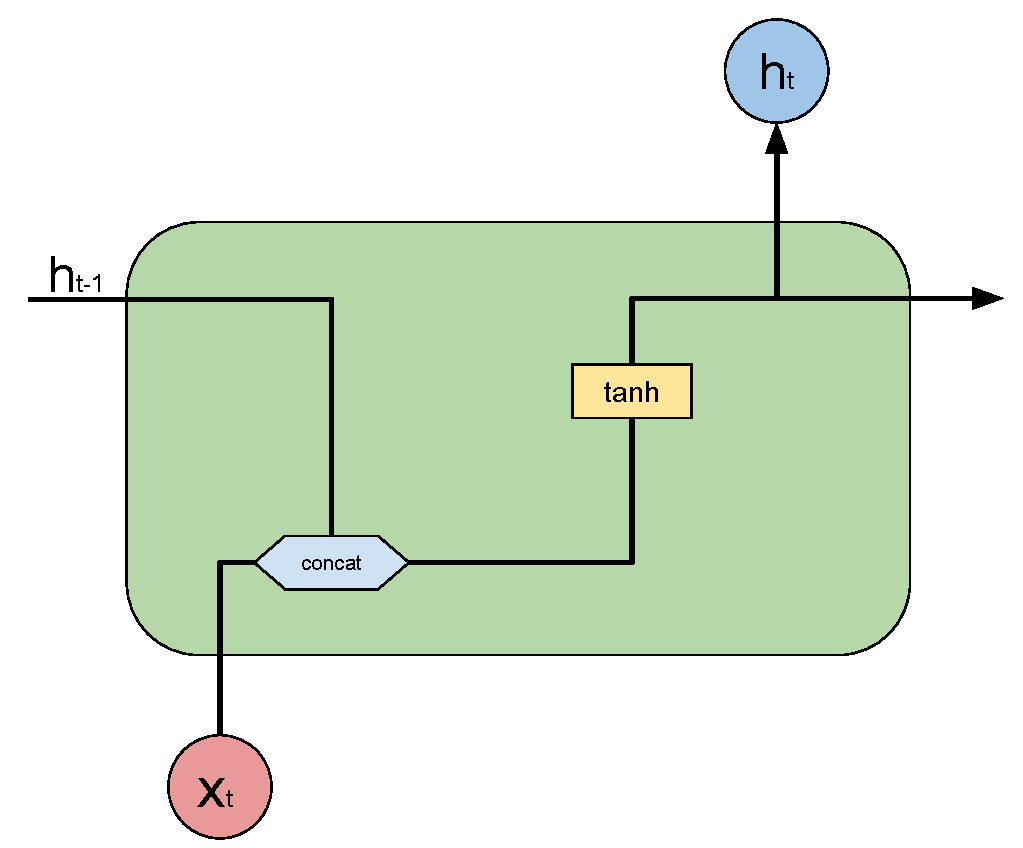
\includegraphics[width=\textwidth]{images/RNN_cell_simple.pdf}
        \caption{Vanilla RNN cell}
        \label{subfig:rnn_cell}

    \end{subfigure}%
    ~ 
    \begin{subfigure}[t]{0.5\textwidth}
        \centering
        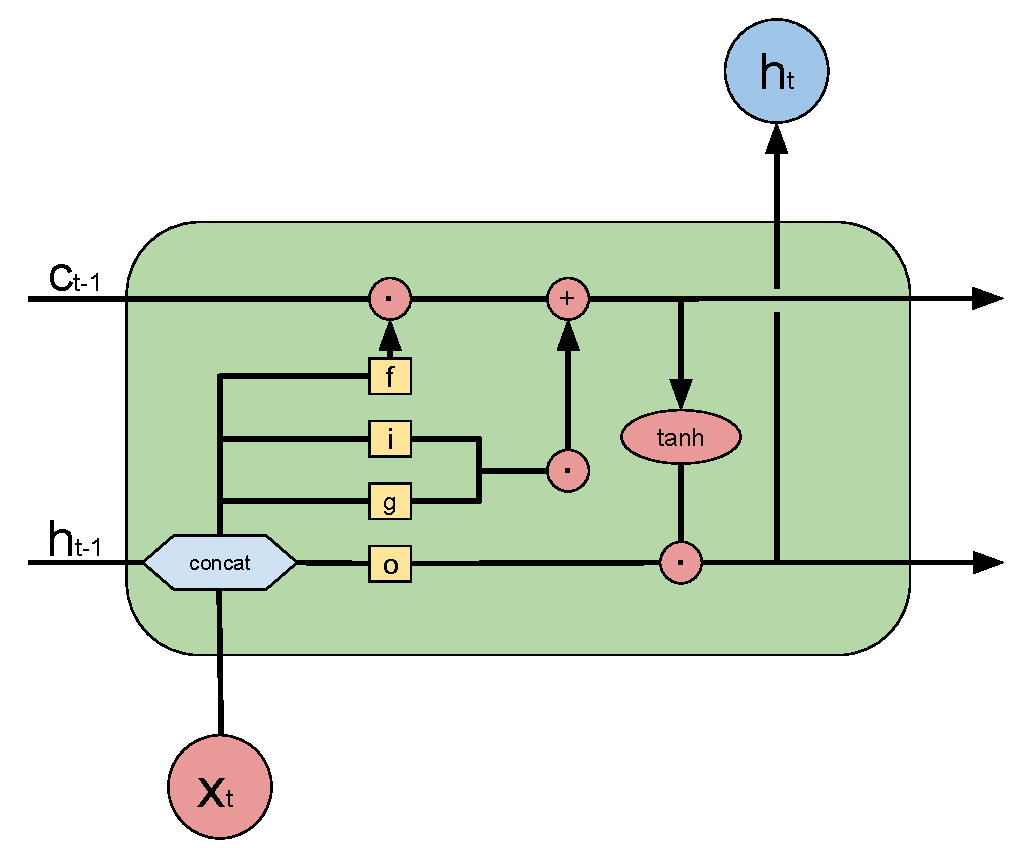
\includegraphics[width=\textwidth]{images/LSTM_cell_simple.pdf}
        \caption{LSTM cell}
        \label{subfig:lstm_cell}

    \end{subfigure}
    \caption{Different types of cells. Red circles are for point-wise operations, in yellow we have neural networks.} % activation functions (these can be seen as neural network, where the weights are in W, and they use different parts of W). } % The blue circle is the dot product, and the stack operation creates a n-dimensional vector with n as the number of input elements.}
    \label{fig:cells}
\end{figure} 

\paragraph{}
Long Short Term Memory networks (LSTM) are an improved version of RNNs  that introduces mechanisms to decide what should be ``remembered" and ``forgotten". Proposed by~\cite{hochreiter1997long}, LSTMs are a solution to the long-term dependencies issue in vanilla RNN and the vanishing of the gradient. LSTMs mitigate the problem by having a more complex cell that contains two hidden states. The first one is $h_t$ and is similar to the one in RNNs, the other is $C_t$, the cell state, which is the core of a LSTM cell. The cell state is modified using the gates, which are neural networks acting on the information of the cell state and the hidden state. In Figure~\ref{fig:cells} we can see how the information flows and interact with the different gates, these are:

\begin{itemize}[-]
    \item Forget gate layer ($f$): acts on what and how much to forget from the previous time step. It is computed using a neural network with a sigmoid $\sigma$ activation function. The output of the network is between 0 and 1, since the output will be multiplied element-wise 0 means forget all, and 1 remember all. $f_t = \sigma(W_f * [h_{t-1}, x_t])$;
    \item Input gate layer ($i$): this gate decides which information to write to the cell state. It is a sigmoid layer: $i_t = \sigma(W_i * [h_{t-1}, x_t])$, and works in combination with the gate layer; 
    \item Gate gate layer ($g$): decides how much to write to the cell state. It is a $\tanh$ layer, $g_t = \sigma(W_g * [h_{t-1}, x_t])$. The output is the multiplied by the input gate output to create a new candidate state cell that will be summed with the value of the previous cell state after the forget step. The new cell state is  $c_t = f_t \odot c_{t-1} + i_t \odot g_t$;
    \item Output gate layer ($o$): this layer is responsible of how much of the cell state to reveal through the hidden state. This is done using a sigmoid layer which decides the parts of the cell state that will be shown in the output, formally $o_t = \sigma(W_o * [h_{t-1}, x_t])$. Then, we put the cell state through $\tanh$ (to push the values to be between −1 and 1) and multiply it by the output of the output layer, so that we only expose the parts we decided to. Formally, the hidden state will be $h_t = o_t \odot \tanh(c_t)$.
\end{itemize}


% The previous equations can be wrote more compactly as show in Equation~\ref{eq:lstm}. We have $W \in \mathbb{R}^4$, where each element is a matrix of weights for the different layers of the cell. The hidden layer $h_t$ and the input $x_t$ are both vectors. And $\sigma$, $tahn$ are the activation functions. 

% \begin{equation}
% \begin{split}
%          W & = [W_i, W_f, W_o, W_g] \\ 
%          \begin{bmatrix}
%           i \\
%           f \\
%           o \\
%           g   
%         \end{bmatrix} & =         \begin{bmatrix}
%           \sigma \\
%           \sigma \\
%           \sigma \\
%           \tanh
%          \end{bmatrix}  W   \left[ h_{t-1}, x_t\right]\\
%          c_t & = f \odot c_{t-1} + i \odot g \\
%          h_t & = o \odot \tanh(c_t) \\
% \end{split}
% \label{eq:lstm}
% \end{equation}

This is the general LSTM; however there are many variants of LSTMs, which perform slightly better or worse depending on the task. A more detailed work on how each variant perform is ``LSTM: A Search Space Odyssey" by~\citet{greff2017lstm}.


\subsection{Attention mechanism}
\label{sec:encoder_decoder}


\paragraph{}
A very popular RNN architecture is the sequence-to-sequence, or encoder-decoder ~\citep{cho-etal-2014-learning,sutskever2014sequence}. This framework is very popular in many NLP tasks, including neural machine translation, text summarization, question answering, and many more. 
% \begin{wrapfigure}{r}{0.5\textwidth}
%         \centering
%         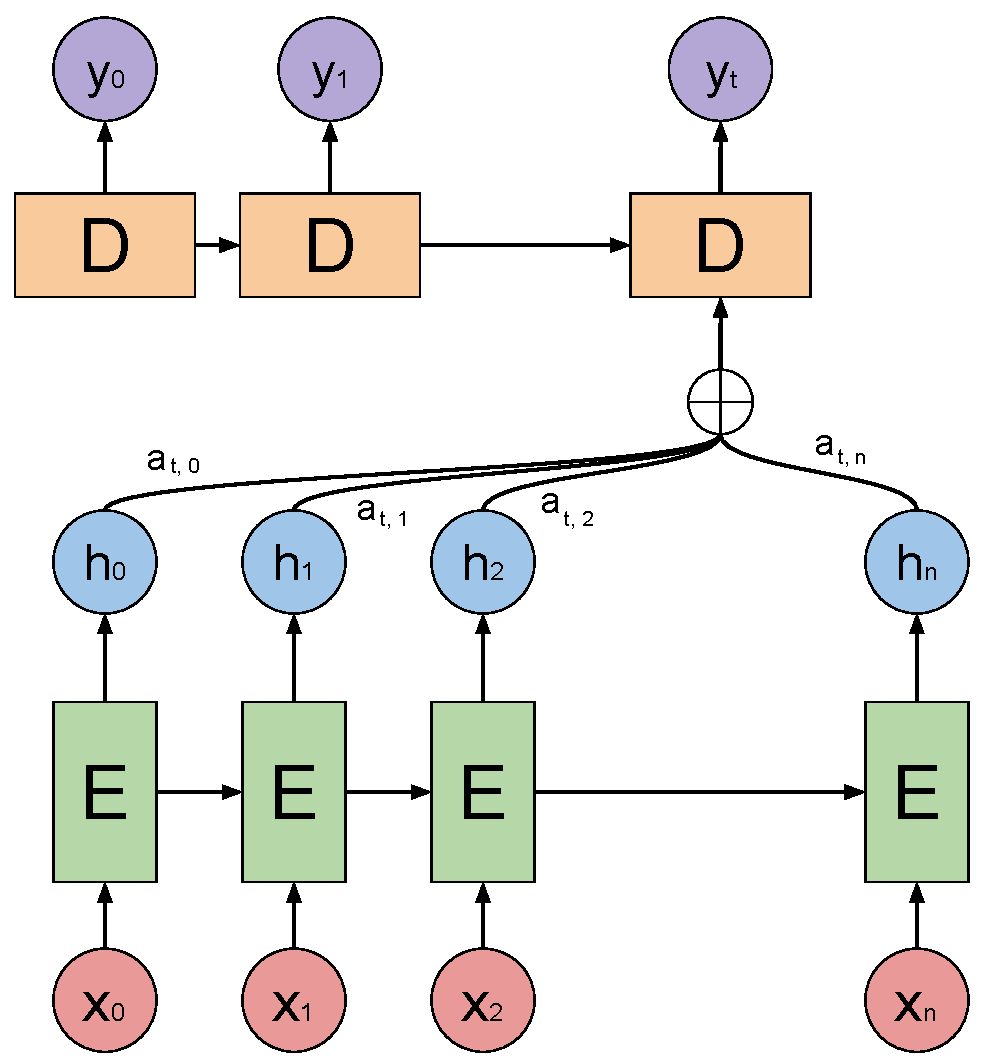
\includegraphics[width=0.5\textwidth]{images/Attention.pdf}
%         \caption{Attention mechanism. The encoder $E$ hidden states are used as input to the decoder $D$ to produce the output of at step $t$.}
%         \label{fig:attention}
% \end{wrapfigure}%

A sequence-to-sequence model is composed by an encoder, which takes the input sequence and compresses it into a context vector which will be used to start the decoder which predicts an output sequence.  A significant and clear disadvantage of a fixed-size context vector design is as the sequence gets longer and longer, more memory is required to store past information but the encoder is unable to represent all of it due to the fixed dimension of the vector. As a result, the network performs poorly on longer sequences~\citep{cho-etal-2014-properties}. A solution to this has been proposed by~\cite{bahdanau2014neural}, by introducing an attention mechanism for the decoder, instead of just relying on the previous hidden state, the decoder with attention can use information from all the input sequence by looking at the encoder hidden state at each time step and combine this information to produce the output.

\paragraph{Encoder:} Given a sequence of vectors $\textbf{x} = (x_1, \dots, x_n)$, an RNN takes this sequence and produces a context vector $c$:

\begin{equation}
    \begin{split}
        h_t & = f(x_t, h_{t-1})\\
        c & = q(\{h_1, \dots, h_n\}) 
    \end{split}
\end{equation}

where $h_t$ is the hidden state at time $t$, and $f$ and $q$ are nonlinear functions. Some example of $f$ and $g$ include: LTSMs for $f$, and return the last hidden state for $g$. This part is the same with or without attention mechanism.



\paragraph{Decoder:} Given a context vector, the decoder computes the probability of a sequence $\textbf{y} = (y_1, \dots, y_T)$ by decomposing the joint probability into the ordered conditionals to the context vector, and the previous outputs.

\begin{equation}
P(\mathbf{y})=\prod_{t=1}^{T} P\left(y_{t} |\left\{y_{1}, \cdots, y_{t-1}\right\}, c\right)
\end{equation}

Which can be implemented using RNNs, where $g$ is a nonlinear function, and $s_t$ is the decoder hidden state:

\begin{equation}
P(\mathbf{y})=\prod_{t=1}^{T} g\left(y_{t-1}, s_{t}, c\right)
\end{equation}


\begin{figure}[t]
        \centering
        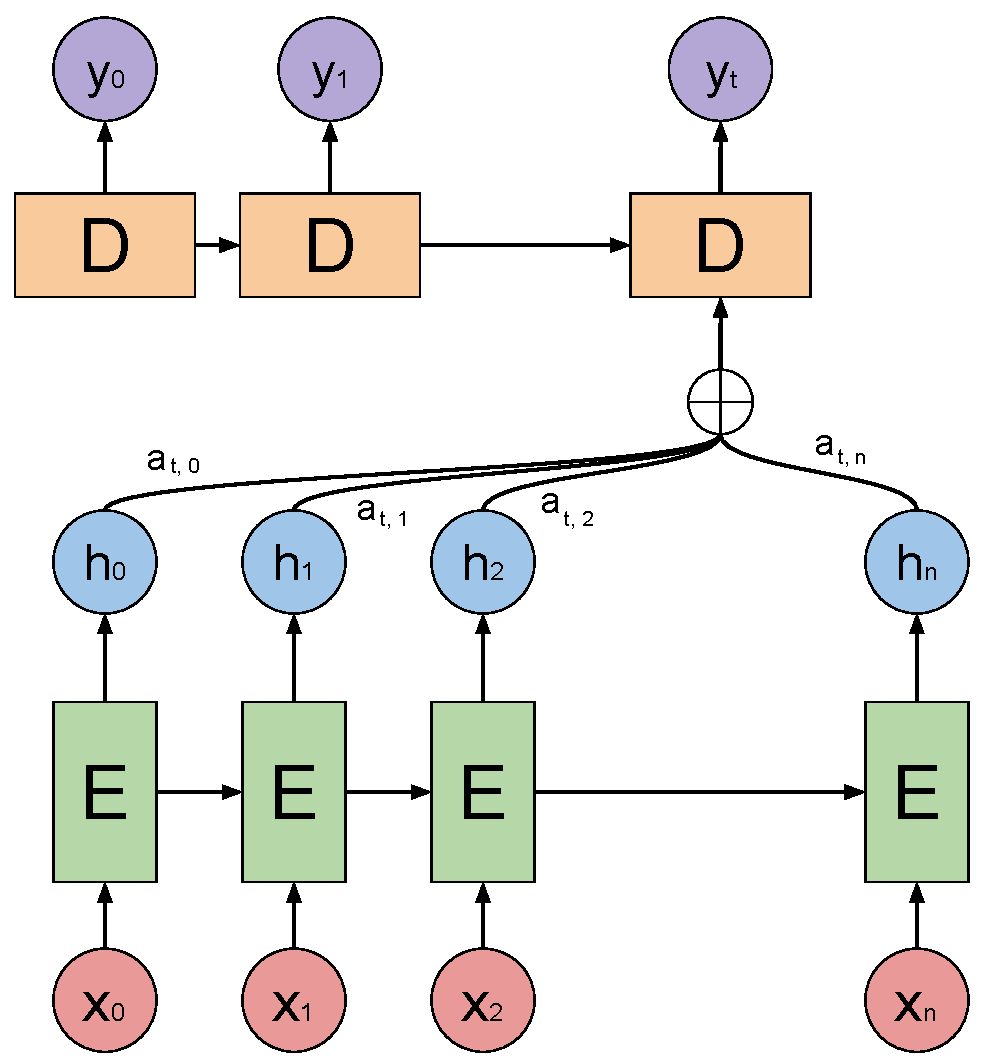
\includegraphics[width=0.5\textwidth]{images/Attention.pdf}
        \caption{Attention mechanism. The encoder $E$ hidden states are weighted via $a_{i, j}$, summed, and used as input to the decoder $D$ to produce the output at step $t$.}
        \label{fig:attention}
\end{figure}%

\paragraph{Decoder with Attention:} Illustrated in Figure~\ref{fig:attention}, the \cite{bahdanau2014neural} decoder performs the same task as the before, but instead of being conditioned to the context vector and the previous output, the probability of each output is conditioned to the previous outputs, and the entire input sequence.



\begin{equation}
P(\mathbf{y})=\prod_{t=1}^{T} P\left(y_{t} |\left\{y_{1}, \cdots, y_{t-1}\right\}, \textbf{x}\right) = \prod_{t=1}^{T} g\left(y_{t-1}, s_{t}, c_t\right)
\end{equation}

The new context vector is computed as a weighted sum of the encoder hidden state $(h_1, \dots, h_n)$: 

\begin{equation}
\begin{split}
    c_{i} & = \sum_{j=1}^{n} \alpha_{i j} h_{j}\\
    \alpha_{i j} &= \frac{\exp \left(e_{i j}\right)}{\sum_{k=1}^{n} \exp \left(e_{i k}\right)} \\
    e_{i j} &= a\left(s_{i-1}, h_{j}\right)
\end{split}
\end{equation}

The weight $\alpha_{i j}$ is a probability that indicates the importance of the $j$-th encoder state $h_j$ with regard to the previous decoder hidden state $s_{i-1}$ to produce the next hidden state $s_i$ and the output of $y_i$ . The weights are computed using a neural network $a$ called alignment model, since~\cite{bahdanau2014neural} proposed this architecture in a neural machine translation task, and the idea behind it is to find which words in the source sequence are more relevant to predict the output by effectively learning to align the source sentence with the target one. Having the decoder look at the entire input sequence implements a so-called attention mechanism, which allows the encoder to decide at which part of the input to attend.  By letting the decoder have this mechanism, we reduce the encoder responsibility of having to encode all information in the source sequence into a fixed length vector since the decoder can selectively retrieve the useful information in the sequence accordingly to the current state needs.

Even if attention can be used as an interpretation method for machine translation, \citet{sarthak2019attention} used an adversarial setup and found that there are some tasks like text classification, question answering and natural language inference where the gradient based feature importance measure is not equivalent to the attention weights, and it is also possible to train new weights of the attention mechanism while maintaining the same performance and having these new weighs mean nothing to human experts.

The idea of having an attention mechanism became very successful in many other NLP task due to the increase in performance it brings. Its value in NLP inspired a new model, called Transformer~\citep{vaswani2017attention}, which separates the attention mechanism from the RNN, having a framework entirely based on it. 

\subsection{Transformer}

\begin{figure}[h]
        \centering
        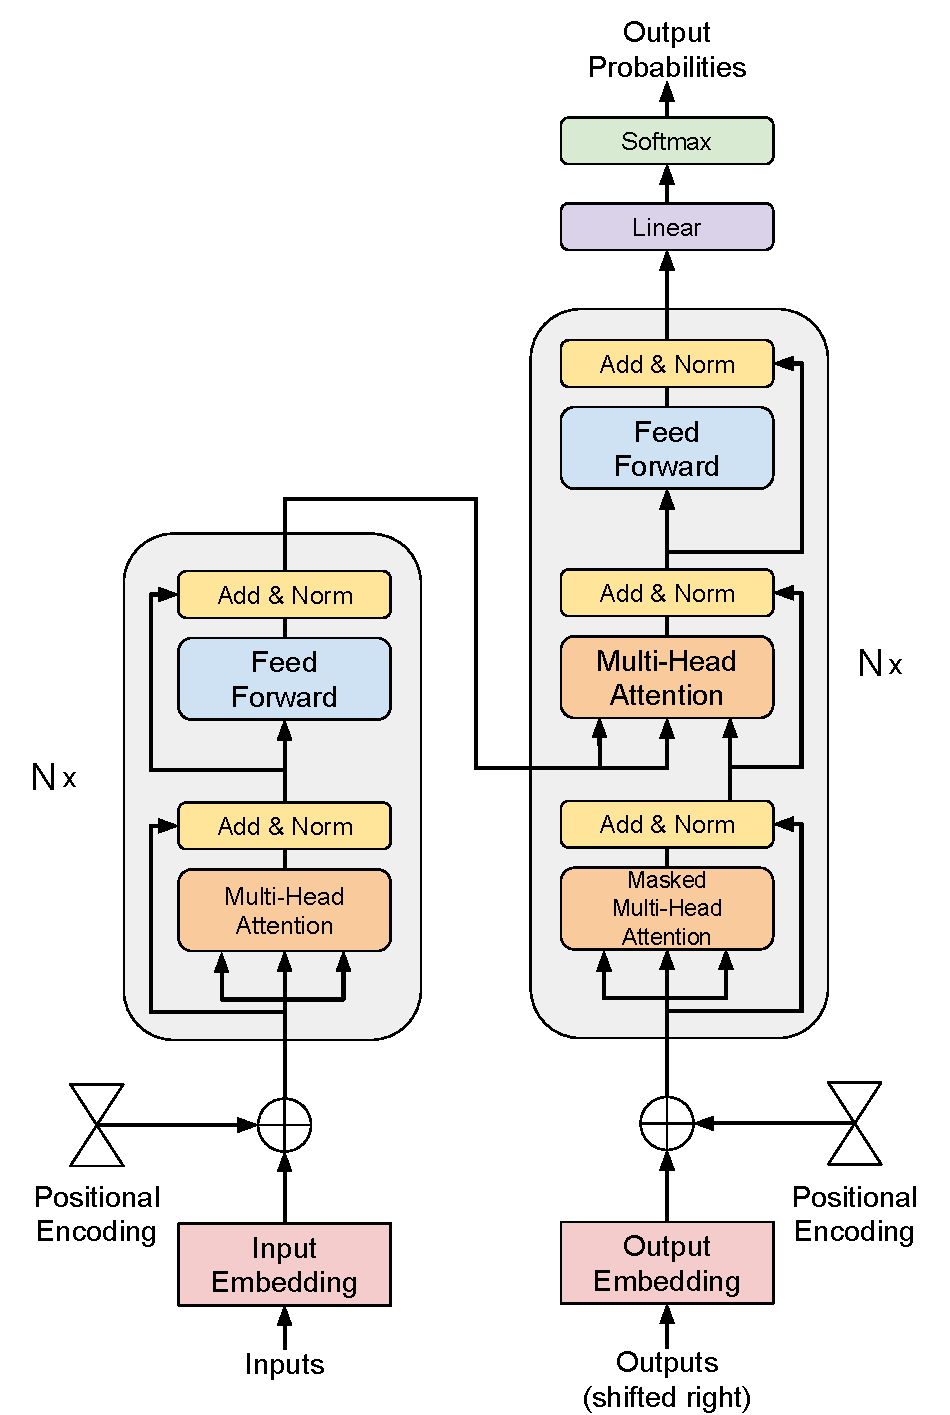
\includegraphics[width=0.5\textwidth]{images/Transformer.pdf}
        \caption{Transformer model architecture.}
        \label{fig:transformer}
\end{figure}

\paragraph{}
Sequence-to-sequence frameworks are state-of-the-art in most of sequence transduction tasks, and almost all of these models use attention mechanism. However, they need sequential computation due to their nature, making models hard to train. \citet{vaswani2017attention} proposes a new framework, the transformer, that still has the same overall encoder-decoder structure, but without recurring networks, allowing their model to be paralleled and making it less needy in terms of resource and computational time while also being able to set new state-of-the-art performance in various tasks.

\citet{vaswani2017attention} also generalize the idea of attention by proposing a new formalization. According to them, the attention is a function that maps a query $Q$ and a set of key-value pair $\langle K, V\rangle$ to an output. The output is a weighted sum of the values. The weight is assigned by computing the compatibility function of the query with the corresponding key. In terms of the definition of \citet{bahdanau2014neural} we have that the query is the decoder hidden state ($s_j$), the keys are the encoder hidden state ($h_j$), and the values are the hidden states of the encoder. \citet{vaswani2017attention} uses a so called scaled-dot product attention (Equation~\ref{eq:dot-attention}), while the one that used by \cite{bahdanau2014neural} is called additive or concat attention, but there are many others.

\begin{equation}
    Attention\left(Q, K, V\right) = softmax\left(\frac{QK^\intercal}{\sqrt{d_k}}\right)V
    \label{eq:dot-attention}
\end{equation}

The transformer has a stack of $N$ encoders (left part of model in Figure~\ref{fig:transformer}), and also $N$ stacks of decoders (right side of Figure~\ref{fig:transformer}). A stack is made up by different sub-layers. 

\paragraph{Encoder:} it has two sub-layers, a multi-head self attention one and a feed forward neural network. Each sub-layer has residual connection~\citep{he2016residual} and, layer normalization~\citep{lei2016normalization}. The output of each sub-layer is $LayerNorm(x + Sublayer(x))$.

\paragraph{Decoder:} it has the same sub-layers as the encoder plus an extra one that performs multi-head attention over the encoder output. The first attention layer is changed to perform a masked version of attention, forcing the prediction at time $t$ to be dependant only on the know outputs.

\paragraph{}
A big part of the transformer is the multi-head attention (Equation~\ref{eq:multi_attention}). The transformer computes $h$ different attentions. The attentions are computed by projecting the query $Q$, the keys $K$, and the values $V$ $h$ different times resulting in $h$ different attention heads exhibiting different behaviours that seems related to the sentence  structure making each head learn a different task (e.g. anaphora resolution). The heads are then concatenated and projected one last time to get the final result. There are two types of attention in the transformer: the regular encoder-decoder attention, and the self attention. Self-attention, or intra-attention~\citep{cheng-etal-2016-long}, is an attention mechanism relating different positions of a single sequence in order to compute a representation of it, it is used between the sub-layers of both the encoder and the decoder, allowing all the position to attend over all other tokens in the sequence. 

\begin{equation}
    \begin{split}
        MultiHead(Q, K, V) & = Concat\left(head_{1}, \ldots,  head_{h}\right) W^{O} \\
        head_{i} & = Attention \left(Q W_{i}^{Q}, K W_{i}^{K}, V W_{i}^{V}\right)
    \end{split}
    \label{eq:multi_attention}
\end{equation}

There are state-of-the-art solutions that use the transformer as their construction core, some of these solution are beating multiple NLP challenges without changes to their architecture. A couple examples are BERT~\citep{devlin2018bert}, and OpenAI GPT~\citep{radford2018improving}. 

The transformer has also some major drawback, the perk of being parallelizable comes at the cost of loosing the recurrent inductive bias of RNNs, which seems to be essential for generalizing on different sequence modeling tasks of varying complexity. The transformer is also not Turing complete, and lacks conditional processing of the input sequence. Some proposed solution are the Transformer-XL~\citep{dai2019transformerxl} and the Universal Transformer~\citep{dehghani2018universal}. 

\section{Word Representation}
\label{sec:word_embedding}
\paragraph{}
Word representation is an elemental part of most Natural Language Processing (NLP) tasks. The understanding of text is mainly derived by transforming text into usable computational representations, these include graphs, trees, or vectors on which will the focus.   In general, it has been found to be beneficial to represent words or documents as vectors, which have an appealing, intuitive interpretation, and they capture hidden information concerning a language, like word analogies or semantic. 
%A word representation is a mathematical object associated with each word, often a vector.

% Based on the literature \citep{turian2010word, schnabel2015embeddings},  \cite{almeida2019word} define word embeddings as a e dense, distributed, fixed-length word vectors, built using word co-occurrence statistics as per the distributional hypothesis

A very simple way to transform words into vectors is the one-hot-encoding which consist of having a vector for each word in the vocabulary, the vectors are of size equal to all the words in the vocabulary. This vector will have all entries at 0, except for one which will be the position representing the word, which will be set to 1. 

There are various methods to induce more meaningful word representation, the two main types are count based and prediction based approaches~\citep{baroni-etal-2014-dont}. Or following~\cite{turian2010word} distributional and distributed representation respectively.


\begin{itemize}[- , itemsep = 0.1em]
\item Count based: are based on co-occurrence context and on the distributional hypothesis:  ``\textit{linguistic items with similar distributions have similar meanings}", hence the similarity is expressed in terms of the similarity of the distribution. Traditional solutions include the creation of a spare matrix containing the association of the word with a context. An example of association is the Pointwise Mutual Information (PMI). The problem with this sparse representation is that become computational inefficient, solution like Singular Value Decomposition help with the reduction of these high dimensional and spare matrices. An important example of count based approach is GloVe~\citep{pennington2014glove} which we will describe in the next paragraphs.

\item Prediction based: 
The model learn representations by trying to predict the token given the context, or vice versa. Some examples include the work of \citet{collobert2008a} which for the first time demonstrated the utility of word embeddings for downstream tasks and their proposed neural network architecture forms the foundation for many current approaches, and the Word2Vec framework ~\citep{mikolov2013models,mikolov2013distributed} which popularized word embeddings.
\end{itemize}

\cite{levy-etal-2015-improving} shows that both count and prediction methods have the same performance, without one overtaking the other.


In the work ``\textit{Word representations: A simple and general method for semi-supervised learning}", \citet{turian2010word} define as ``\textit{word embeddings}" only the distributed representation (prediction based), but over time this distinction is not enforced and is common to refer to all vector word representations as word embeddings. 

% \begin{itemize}[itemsep = 0.1em]
% \item Distributional word representation: are based on co-occurrence context and on the distributional hypothesis:  ``\textit{linguistic items with similar distributions have similar meanings}", hence the similarity is expressed in terms of the similarity of the distribution. Some common representation techniques include Latent Semantic Analysis~\citep{deerwester1990indexing} and Latent Dirichlet Allocation~\citep{bei2003lda}. An important example is the work of \citet{pennington2014glove} which propose a competitive set of pre-trained word representations, his work signals that word representation had reached the main stream.

% \item Distributed representation: are compact, dense and low dimensional representation, where each dimension of the embeddings represents a latent feature of the word, hopefully capturing useful syntactic and semantic properties. A distributed representation is compact, in the sense that it can represent an exponential number of clusters in the number of dimensions. Some examples include the work of \citet{Collobert2008} which for the first time demonstrated the utility of word embeddings for downstream tasks and their proposed neural network architecture forms the foundation for many current approaches, and the Word2Vec framework ~\citep{mikolov2013models,mikolov2013distributed} which popularized word embeddings.
% \end{itemize}

% In the work ``\textit{Word representations: A simple and general method for semi-supervised learning}", \citet{turian2010word} define as ``\textit{word embeddings}" only the distributed representation, but over time this distinction is not enforced and is common to refer to all vector word representations as word embeddings. In~\cite{levy-etal-2015-improving} they show how both distributed and distributional methods have the same performance, without one overtaking the other.


\paragraph{}
Another essential part of NLP is the study of language models. A language model is a statistical model of language usage. It consists mainly of predicting the next word given some previous words. A language model learns the probability of word occurrence based on examples of text. Simpler models may look at a context of a short sequence of words, whereas larger models may work at the level of sentences or paragraphs.

More formally, the goal of a statistical language model is to learn the probability $P(x_1, \dots, x_m)$ for a sequence of tokens $x_1, \dots, x_m$. We can compute this via the chain rule of probability:

\begin{equation}
P\left(w_{1}, \ldots, w_{m}\right)=\prod_{i=1}^{m} P\left(w_{i} | w_{1}, \dots, w_{i-1}\right)
\end{equation}

Because the number of words that precede a word varies, and because it is difficult to compute $P(w_i | w_1,\dots, w_{i-1})$ with $i$ large, we typically condition the probability of a word on a window of n previous words ($n$-grams): 


\begin{equation}
P\left(w_{1}, \ldots, w_{m}\right) \approx \prod_{i=1}^{m} P\left(w_{i} | w_{i-n}, \dots, w_{i-1}\right)
\end{equation}

Unfortunately, this approach doesn't generalize to new sequences, unless using some tricks like~\citet{katz1987probablm} did where he computes small $n$-grams, generally $n=3$, and then generalizes to unseen sequences by producing new ones using overlapping $n$-grams of length up to $n$. However, this solution does not generalize to sequences longer than $n$, which has to be small, and also does not take in consideration the similarities of words. Moreover, statistical language models suffer from the problem known as curse of dimensionality that appears when the vocabulary size increases. For example, computing the joint probability of 10 consecutive words having a vocabulary size of 100k there are $100000^{10} - 1 = 10^{50} - 1$ free parameters. 

\citet{bengio2000nnlm} developed a solution for the course of dimensionality of statistical language models by proposing the first large-scale language model based on neural networks, referred to as Neural Network Language Models (NNLMs). In their work \citet{bengio2000nnlm} bring together language modeling and word embeddings by \begin {enumerate*} [1) ]
\item associating each word in the vocabulary with a distributed word vector called ``\textit{feature vector}" \item express the joint probability function of word sequences in terms of the feature vectors of these words in the sequence; \item learn simultaneously the word feature vector and the parameters of the probability function.
\end {enumerate*} This new representation also generalizes to longer sequences and is able to learn similarities between words. \citet{bengio2000nnlm} conclude their work by suggesting the use of Recurrent Neural Networks (RNN) to take advantage of temporal structures and also consider longer sequences like entire paragraphs.

A few years later, \citet{Mikolov2010RecurrentNN} propose a neural language model based on RNN. They use a vanilla RNN~\citep{elman1990finding} to show how language models based on recurrent networks are significantly better that previous solution. They perform experiments on various speech recognition task, and achieve better results even when training using lower amount of data.

This work and the one of \cite{bengio2000nnlm} were followed by many other word embeddings solutions that build upon their methods, in particular current state-of-the-art solutions use RNN, or improved versions like Long Short Term Memory networks~\citep{hochreiter1997long}. There are two types of embeddings, the first one is general embeddings which are not dependent on the context like Word2Vec~\citep{mikolov2013models,mikolov2013distributed}, GloVe~\citep{pennington2014glove}, and fastText~\citep{bojanowski2016enriching}; the second is context dependent embeddings, these are the new state-of-the-art solution and include ELMo~\citep{peters2018elmo}, and BERT~\citep{devlin2018bert}. We will present fastText and BERT in Section~\ref{sec:w_e} since are the embeddings we compare for our solution. Now, we will present Word2Vec, GloVe, and ELMo.


\paragraph{Word2Vec} \cite{mikolov2013models} proposes two log-linear models, the skip-gram (SG), and the Continuous Bag-of-Words (CBOW). Skip-gram model trains a network to predict the word given the context in which the word appears. While the CBOW does the inverse, it predicts the context of a word given that word. The network is a feedforword neural network with one hidden unit. We have an input layer which is projected onto a hidden layer using a matrix $W$, the word embeddings matrix, then the hidden layer is projected to the output layer using a matrix $\tilde{W}$, which is the word context embeddings. 

Given a corpus $\mathcal{C}$, a vocabulary $V$, a context of size $n$, and a word $x_t$, we define the skip-gram as follows:

\begin{equation}
J_{\mathrm{SG}}=-\frac{1}{|\mathcal{C}|} \sum_{t=1}^{|\mathcal{C}|} \sum_{-n \leq j \leq n, j \neq 0} \log P\left(x_{t+j} | x_{t}\right)
\end{equation}

while the CBOW:

\begin{equation}
J_{\mathrm{CBOW}}=-\frac{1}{|\mathcal{C}|} \sum_{t=1}^{|\mathcal{C}|} \log P\left(x_{t} | x_{t-n}, \dots, x_{t-1}, x_{t+1}, \dots, x_{t+n}\right)
\end{equation}

Both probabilities are computed using the softmax function:

\begin{equation}
\frac{\exp \left(\tilde{\mathbf{w}}_{z}^{\top} \mathbf{w}_{s}\right)}{\sum_{j=1}^{|V|} \exp \left(\tilde{\mathbf{w}}_{j}^{\top} \mathbf{w}_{s}\right)}
\end{equation}

where $\mathbf{w_i} \in W$, $\mathbf{\tilde{w}_i} \in \tilde{W}$ are the word and context embeddings for word $x_i$ and can be extracted by multipling the one-hot-encoding of word $x_i$ with matrix $W$ and $\tilde{W}$ respectively. For the SG $\mathbf{w}_s = \mathbf{w}_t, \mathbf{w}_z = \mathbf{w}_{t+1}$ , and for the CBOW $\mathbf{w}_s = \sum_{-n \leq j \leq n, j \neq 0} \mathbf{w}_{t+j}, \mathbf{w}_z = \mathbf{w}_{t}$.  This is very inefficient, since for each prediction we need to iterate over the entire vocabulary. An improved version of the softmax is the hierarchical softmax~\citep{Morin05hierarchicalprobabilistic}, which uses a tree structure to reuse already computed probabilities, bringing the complexity to $O(log(|V|))$, with the softmax complexity equals to $O(|V|)$.

In a following work, ~\cite{mikolov2013distributed} propose an efficient way to train NNLMs, called negative sampling, a simplified version of noise contrastive estimation ~\citep{gutmann2012contrastive}. Negative sampling trains the model to distinguish
a target word $w_{t+1}$ from negative samples drawn from a noise distribution $P_z$. Negative sampling is defined as:

\begin{equation}
P\left(x_{t+j} | x_{t}\right)=\log \sigma\left(\tilde{\mathbf{w}}_{t+j}^{\top} \mathbf{w}_{t}\right)+\sum_{i=1}^{k} \mathbb{E}_{w_{i} \sim P_{z}} \log \sigma\left(-\tilde{\mathbf{w}}_{i}^{\top} \mathbf{w}_{t}\right)
\label{eq:neg_samp}
\end{equation}

where $\sigma$ is the sigmoid function and $k$ is the number of negative samples. This can be easily adapted also for the CBOW.

~\cite{levy2014embedding_pmi} show how SG with negative sampling is an implicit factorization of the Pointwise Mutual Information matrix, which is a count based        method.

\paragraph{GloVe} 
Global Vector~\citep{pennington2014glove} is a embedding method based on co-occurrence matrix factorization. GloVe use a co-occurrence matrix $C$, where an entry $C_{ij}$ is the number of times word $x_i$ appears in the context of word $x_j$. They use it to compute a probability matrix $P$ of a word of being in the context of another word, where $P_{ij}$ is the probability of word $x_i$ being in the context of word $w_j$. The main idea is that word meanings are captured by the ratios of co-occurrence probabilities rather than the probabilities themselves, they want to model a function $F$ that is able to approximate this ratio using the word vectors, and context word vectors.

\begin{equation}
F\left(\mathbf{w}_{i}, \mathbf{w}_{j}, \tilde{\mathbf{w}}_{k}\right)=\frac{P_{i k}}{P_{j k}}
\end{equation}

To preserve the information of the probability ratio, and maintain the linear structure, the previous equation becomes: 

\begin{equation}
F\left(\left(\mathbf{w}_{i}-\mathbf{w}_{j}\right)^{T} \tilde{\mathbf{w}}_{k}\right)=\frac{P_{i k}}{P_{j k}}
\end{equation}

They find that the best candidate for $F$ is the $exp$ function, and via various step, they obtain the following error function:
\begin{equation}
    \mathbf{w}_{i}^{T} \tilde{\mathbf{w}}_{j}+b_{i}+\tilde{b}_{j}-\log C_{i j}
\end{equation}

where the $b_i$ and $\tilde{b}_j$ are bias terms. The only problem with this equation is word with low frequency are treated in the same way as the one with high frequency, to fix this they add an weight function $f$ with some conditions. The final cost function is:

\begin{equation}
J_{GloVe} = \sum_{i, j=1}^{|V|} f\left(C_{i j}\right)\left(\mathbf{w}_{i}^{T} \tilde{\mathbf{w}}_{j}+b_{i}+\tilde{b}_{j}-\log C_{i j}\right)^{2}
\end{equation}

\paragraph{ELMo} Proposed by ~\cite{peters2018elmo}, it is a deep contextualized word representation model. Instead of having a fixed embedding that represents a word, contextualized embeddings are a function of the input sequence and are able to model information like polysemy.

ELMo uses a bidirectional language model (biLM) on top of which a task specific representation is created. The contextualized representation is a function of the hidden states of the biLM. Given a biLM with $L$ layers, it computes a set of $2L+1$ representations for each token $t_k$:

\begin{equation}
\begin{split}
R_{k} & =\left\{\mathbf{h}_{kj}^{LM},| j=0, \ldots, L\right\}    
\end{split}
\end{equation}
 

where $h_{k0}^{LM} = x_k^{LM}$ (the token representation from the language model), and $h_{kj} = [\overrightarrow{\mathbf{h}}_{k j}^{LM}, \overleftarrow{\mathbf{h}}_{k j}^{L M}]$. Then a task specific representation is computed.

\begin{equation}
\mathbf{E} \mathbf{L} \mathbf{M} \mathbf{o}_{k}^{task}=E\left(R_{k} ; \Theta^{task}\right)=\gamma^{t a s k} \sum_{j=0}^{L} s_{j}^{task} \mathbf{h}_{k, j}^{LM}
\end{equation}

where  $E$ is a function for creating task specific embeddings parametrized by $\Theta$. An generic example is the weighted sum. The weights $s^{task}$ in the linear combination are learned for each end task and normalized by softmax. The scaling factor $\gamma^{task}$ is used to correct the misalignment between the distribution of the biLM hidden states and the distribution of task specific representations.



\section{Transfer Learning}
\label{sec:transfer_learning}

\paragraph{}
In this section we will introduce the definition and the types of transfer learning based on the survey of~\cite{pan2010transfer}, and the thesis of~\cite{ruder2019neural} in which he applies transfer learning techniques to NLP. We will start with the general definition of transfer learning, present an overview of the different types, and then focus our attention on the techniques we will use in our work. 


\subsection{Introduction}
\paragraph{}
In the traditional supervised scenario, the availability of training data is not always guaranteed; in some cases, the number of accessible data of the target domain is scarce, or entirely lacking. Deep neural networks suffer from the unavailability of data even more opposed to more traditional machine learning algorithms. Transfer learning relaxes the hypothesis that training data and test data must be independent and identically distributed (i.i.d assumption), allowing the use of data of a \textit{source domain} and a task on this data, known as \textit{source task}. The knowledge from the source domain, and source task is used as a background knowledge when solving the \textit{target task} from a \textit{target domain}. 

Formally, a domain $\mathcal{D}$ is made by two components $\mathcal{D} = \{\mathcal{X}, P(X)\}$, where $\mathcal{X}$ is a feature space, $P(X)$ is a marginal probability distribution over a feature space, and $X = \{x_1, \dots, \x_n\} \in \mathcal{X}$. Given a domain, a task $\mathcal{T}$ 
consists of a label space $\mathcal{Y}$, a prior distribution $P(Y)$, a conditional probability distribution $P(Y|X)$. 

Given a source domain $\mathcal{D}_S$ and learning task $\mathcal{T}_S$, a target domain $\mathcal{D}_T$ and learning task $\mathcal{T}_T$, transfer learning aims to help improve the learning of the target conditional probability $P_T(Y_T|X_T)$ in $\mathcal{D}_T$ using the knowledge from $\mathcal{D}_S$ and $\mathcal{T}_S$, where $\mathcal{D}_S \neq \mathcal{D}_T$, or $\mathcal{T}_S \neq \mathcal{T}_T$.

Since the domain and task are tuples, the inequality conditions in the transfer learning definition allows for for five different scenarios grouped in two major settings:

\begin{enumerate}[a -]
    \item Inductive learning: the target task is different from the source task, while the source and target domains may or may not be the same. This setting labeled data in the target domain are required to induce a model.
        \begin{itemize}[- ]
            \item $P_S(Y_S) \neq P_T(Y_T)$. The prior distributions are different. 
            \item $P_S(Y_S | X_S) \neq P_T(Y_T, X_T)$. The conditional probability distributions are different, this can be solved with approaches like over-sampling, or SMOTE.
            \item $\mathcal{Y}_S \neq \mathcal{Y}_T$. The target task has different labels. Depending whether the tasks are learned simultaneously or sequentially we have multi-task learning (MTL) and sequential transfer learning respectively.  
        \end{itemize}
    
    \item Transductive learning: the source and target tasks are the same, while the source and target domains are different. In this setting, no labeled data in the target domain are available while a lot of labeled data in the source domain are available.
        \begin{itemize}[- ]
            \item $P_S(X_S) \neq P_T(X_T)$. Known as domain adaptation, the marginal probability of the source and the target are different. This scenario is common in combination with different prior distributions and also different task labels.
            \item $\mathcal{X}_S \neq \mathcal{X}_T$ The feature space between the target and source are different. In NLP, this scenario is referred to as cross-lingual learning or cross-lingual adaptation.
        \end{itemize}

\end{enumerate}

\citet{ruder2019neural} proposes changes at the taxonomy proposed in~\citet{pan2010transfer} by adapting the general transfer learning types to the NLP domain. We can see the adapted taxonomy in Figure~\ref{fig:nlp_transfer_taxonomy}.

\begin{figure}[]
        \centering
        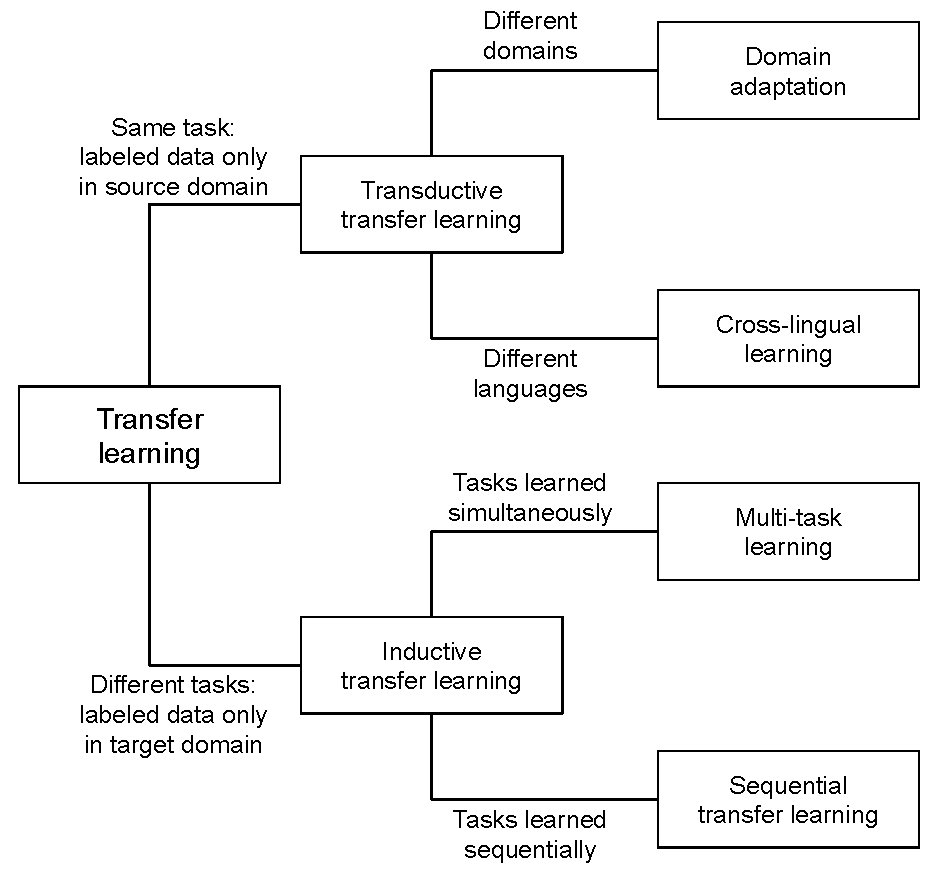
\includegraphics[width=0.5\textwidth]{images/NLP_Transfer_Learning_Taxonomy.pdf}
        \caption{Taxonomy for transfer learning in NLP, as in~\citep{ruder2019neural}}
        \label{fig:nlp_transfer_taxonomy}
\end{figure}%


\subsection{Multi-task Learning}
\paragraph{}
Traditional machine learning problems rely on a single model, which introduce the risk of ignoring critical source of inductive bias. ~\cite{caruana1993mtl} proposes a new learning paradigm based on the idea that related tasks can be used as sources of mutual inductive bias. By introducing this bias, the learning could be faster and more accurate. This approach is called multi-task learning (MTL), or joint learning. 

Given a multitask problem consisting of $m$ tasks $X = \{T_{1}, \dots, T_{m}\}$. For task $T_i$, its training dataset contains $n_i$ examples $X_i = \{x_{i, 1}, \dots, x_{i, n_i}\}$ as well as their labels $Y_i = \{y_{i, 1}, \dots, y_{i, n_i}\}$. The learning function for task $T_i$ is defined as $f_i(x, w_i)$, and $W = \{w_1, \dots, w_n\}$. The function to optimize all the task is:

\begin{equation}
\min_{W} \sum_{i=1}^{m} \frac{1}{n_{i}} \sum_{j=1}^{n_{i}} \mathcal{L}\left(y_{i, j}, f_i(x_{i,j}, w_i)\right) + \lambda\Omega_W
\end{equation}

this means that the goal of the model is to jointly optimize all the tasks, with all of them having the same importance. This could be changed in case we have a main task and the others are auxiliary task, used to help the main model achieve better generalization.

We will present some general works on deep MTL architectures and examples of applications in natural language processing. A type of architecture for MTL consists of a network where the first $n$ layers are shared across all task, and the final layers are task specific. The hard parameter sharing architecture is simple to implement and helps with the reduction of overfitting, but it is only guaranteed to work with closely related task. Another method is the soft parameter sharing, in this case each task has his own layers, and the parameters are then regularized in order to make them similar. 

A more general framework that allows the network to learn what and how much to share across all task are the sluice networks~\citep{ruder2017sluice}. In a sluice network each hidden layer is split in $m$, with $m$ equal to the number of tasks. In a two task setup, we have that each layer is divided in two, one part for the task specific and the other for the sharing of parameters. The communications with the next layer for each task and across tasks is regulated by a two by two matrix with learnable weights. The matrix decides how much information from one task pass to the next layer of the same task, and how much to the next layer of the other task. This reduces the likely of negative transfer.

The use of MTL brings various improvements also in NLP, for example~\cite{collobert2008a} use hard parameter sharing and train a single network on various low level NLP tasks like Part-of-Speech tagging, showing how the general performance of all tasks improves. Moreover, ~\cite{abdou2018semanticmtl} compares different types of parameter sharing techniques, from the hard parameter to the sluice networks showing how semantic parsing task helps other syntactic tasks.


\subsection{Sequential Transfer Learning}
\paragraph{}
Sequential transfer learning is similar to MTL, but instead of having the task learned jointly, we first train one and then the next and so on. This is useful in three scenarios: \begin{enumerate*}[a)]
  \item when the data for the tasks are available at different time
  \item the source task has much more than the target
  \item we need to adapt to various tasks.
\end{enumerate*}

There are different techniques to perform sequential transfer learning, but we will focus on the fine-tuning methods as we use it for our experiments. 

\subsubsection{Fine-tuning}
\paragraph{}
Fine-tuning is a method of adaptation of trained models by updating pretrained models using new data. Is more expensive that other sequential transfer solution like feature extraction, but it requires very little task-specific changes and allows the reuse of more general task to model more specific ones.
Some solution for fine-tuning consists in training a network and then reuse the first $n$ layers for another task by retraining them allowing the gradient to propagate through some or all the layers. This solution is not very effective in all tasks since the model could start forgetting due to the high gradients backpropagating at the beginning of the training phase for the new task. One solution is to gradually unfreeze the layers starting from the higher ones going to the first ones, allowing the gradient to change the task specific layer more drastically than the more general. 

In~\citep{howard-ruder-2018-universal} they propose a method for Universal Language Model Fine-Tuning (ULMFiT) for text classification. Fine-tuning language models has been difficult, due to issues with the required amount of data, and problems with overfitting on smaller dataset or forgetting. ULMFiT solves these problems by proposing novel solutions on like discriminative fine tuning, which manages how the learning rate is set using across different layers, making general layers update less that more specific ones. Moreover, they propose a slanted triangular learning rate, that changes with the number of iteration by first rapidly increase until a specific threshold, at which it decrease slowly. They also use the gradual unfreezing. All these solution allow to train a classifier by just using hundreds of in domain documents.

\subsection{Cross-lingual Learning}
\paragraph{}
Cross-lingual learning aims at extracting information from data in a label-scarce target language by exploiting labeled data from a label-rich language. This is based on the fact that related languages influences each other, meaning that we can extract common information from the corpora of rich languages, and use this information for low-resource ones.  The fundamental challenge of cross-lingual learning stems from a lack of overlap between the feature spaces of source language data and that of target language data, and the availability of parallel resources. 

In the past years, the number of multilingual works has increased, creating more resource and showing increases in performance for various. An example is XNLI, a cross-lingual natural language inference dataset proposed by~\cite{conneau2018xnli} that is used to evaluate textual entailment models. Parallel resources also allow for better multilingual representation, that are effective features for cross-lingual models.

Most of the work on multilingual representation has been on word level, on which we will focus in the next section. However, there are also sentence level representations, such as in~\citep{conneau2018xnli} where they train the target language encoder to represent sentences in the same space as the source language encoder, allowing the transfer.   

\subsubsection{Cross-lingual Word Representation}

Multilingual word representation are a useful way to transfer knowledge across languages. Cross-lingual word representation aims at having a common space where word translations are close. This usually requires some amount of supervision, like small bilingual lexicon, but in the recent years solutions with no supervision appeared~\citep{lample2018translation}.

A simple count based solution that does not require parallel corpora was proposed by~\cite{sogaard2015inverted}, they use Wikipedia as their multilingual corpora and, based on the idea that the same word translated appears in the same Wikipedia articles in the corresponding language, they build an inverted index matrix by taking the articles common across all languages the embeddings will be created. Finally, they perform dimensionality reduction on the inverted indexing matrix.

Another solution consists in aligning the vector spaces of the languages. Word alignments are generally modeled as a linear mapping, which are constrained such that the structure of the initial monolingual spaces is left unchanged. When having a parallel lexicon, one solution~\citep{mikolov2013exploiting} to find a linear transformation can be minimizing:

\begin{equation}
\begin{split}
    W^* & = \argmin_{W \in O_d(\mathbb{R})} ||WX-Y||_\mathbb{F} = UV^{\intercal} \\
    \text{with, } U\Sigma V^\intercal & = SVD(YX^\intercal) 
\end{split}
    \label{eq:word_alignment}
\end{equation}

where $d$ is the size of the embedding, $X$ and $Y$ are the embeddings of the lexicon, one in the source language an the other in the target. The matrix $W$ is an orthogonal matrix of size $d\times d$, this has been shown to lead to better performances~\citep{xing-etal-2015-normalized}, and $||\cdot||_{\mathbb{F}}$ is the Frobenius norm. The translation $t$ of any source word $s$ is defined as $t = \argmax_t cos(W x_s, y_t)$.

% Equation~\ref{eq:word_alignment} can be solved using Singular Value Decomposition (SVD). We can compute $UV^{\intercal}$ as $U\sigma V^{\intercal} = SVD(YX^\intercal)$. 



\section{Zero-shot Learning} 
\label{sec:zero_learning}

\paragraph{}

In this section, we will present an overview of zero-shot learning. It studies how machine learning models could generalize to unseen categories.  In recent years, the number of zero-shot learning methods proposed every year has been increasing rapidly. We will give a description, discuss some general techniques, and show applications in natural language processing tasks. %We will give a definition, present some general ideas behind it, and review some related work applied to NLP.

\subsection{Introduction}
\paragraph{}
Classification is one of the main tasks in machine learning; it is straightforward: given an example consisting of various feature, assign a label to the example. Thus, it has been thoroughly studied in different domains and tasks, from computer vision to natural language processing.  The main issue with this setup is that it does not generalize to new labels. Zero-shot learning~\citep{larochelle2008zeroshot} can be seen as an extreme version of Few-shot learning, and One-shot learning~\citep{miller2002oneshot}.

In their survey, ~\citet{xian2017zero} define the zero-shot learning task as follows: Given a training set $\mathcal{S} = \{(x_1, y_1), \dots, (x_n, y_n)\}$, with $y_i \in Y^{tr}$ the training set classes, the task is to learn a function $f: X \rightarrow Y$ that minimizes the loss function $J(\theta)$,and $F$ is a compatibility function that gives how compatible the input and the label are: 

\begin{equation}
\begin{split}
    \min_{\theta} J(\theta) & = - \frac{1}{N} \sum_{1}^{N} \mathcal{L}(y_i, f(x, \theta)) + \lambda \Omega_\theta \\
    f & = \argmax_{y \in Y} F(x, y; \theta)
\end{split}
\end{equation}

At test time, the aim is to assign to new examples an unseen class label, or in the generalized zero-shot, an unseen or a seen class label. This is achieved by providing the model with a description of each class in some representation, the simplest being a vector of numeric or symbolic attributes.

~\cite{akata2015ale} embeds each class in the space of attribute vectors, their method is called Attribute Label Embedding (ALE). They propose the use of label embeddings as the class description, and train a compatibility function $F$ that minimizes the distance between the label and the image representation. Their $F$ function is:

\begin{equation}
F(x, y ; \theta)=\gamma(x)^{T} \theta \phi(y)
\end{equation}

where $\gamma$ is the input embedding, and $\phi$ the label embedding (e.g word embedding of the image label). 

\subsection{Zero-shot in NLP}
\paragraph{}
Many works in NLP use zero-shot learning methods for different tasks, for example 
\cite{obamuyide-vlachos-2018-zero} perform zero-shot classification using a textual entailment framework called ESIM~\citep{chen-etal-2017-enhanced}. Textual entailment consists of predicting if a sentence, the premise, entails, contradicts or is neutral to another sentence, the hypothesis. By reframing relation classification as a textual entailment task, the text to check if the relation exists is the premise, and the hypothesis is the description of the relation. ESIM is a three-step framework consisting of an input encoding using BiLSTM, a local inference modelling based on attention and vector composition, and the third layer is the inference composition again using the BiLSTM. \cite{obamuyide-vlachos-2018-zero} change the ESIM framework, by using a conditional BiLSTM~\citep{rocktaschel2015reasoning} (cBiLSTM). The cBiLSTM condition the encoding by using the hypothesis encoding as initialization. This allows the model to perform zero-shot classification as the relation information is used in the encoding of the premise.

Another example is for the machine translation task. In~\citep{johnson-etal-2017-googles} they use an encoder-decoder architecture with 8 layer LSTMs and attention mechanism. They enable zero-shot translation by prepending the example strings in the source language with an extra token for the target language and having a shared encoding space for all languages. The same solution is also used in ~\citep{bollmann2019zero} for historical text normalization, with an additional token for the task as they also have an auxiliary task in a multi-task learning setup. 
